%%%%%%%%%%%%%%%%%%%%%%%%%%%%%%%%%%%%%%%%%%%%%%%%%%%%%%%
% A template for Wiley article submissions.
% Developed by Overleaf. 
%
% Please note that whilst this template provides a 
% preview of the typeset manuscript for submission, it 
% will not necessarily be the final publication layout.
%
% Usage notes:
% The "blind" option will make anonymous all author, affiliation, correspondence and funding information.
% Use "num-refs" option for numerical citation and references style.
% Use "alpha-refs" option for author-year citation and references style.

% \documentclass[alpha-refs]{wiley-article}
\documentclass[num-refs]{wiley-article}

% Add additional packages here if required
\usepackage{siunitx}
\usepackage{tcolorbox}
\usepackage{array}
\usepackage{hyperref}
\usepackage{longtable}
\usepackage{geometry}
\usepackage{array}
\usepackage{wrapfig}
\usepackage{lscape}
\usepackage[font=small,format=plain,labelfont=bf,textfont=normal, justification=justified,singlelinecheck=false]{caption}
\usepackage{capt-of}
\usepackage{afterpage}

\newcommand{\squishlist}{%
	\begin{list}{-}%
		{\setlength{\itemsep}{0pt}
			\setlength{\parsep}{0pt}
			\setlength{\topsep}{0pt}
			\setlength{\partopsep}{0pt}
			\setlength{\leftmargin}{1em}
			\setlength{\labelwidth}{1em}
			\setlength{\labelsep}{0.5em}}}
	
\newcommand{\squishend}{\end{list}}

\newcommand{\beginsupplement}{%
	\setcounter{table}{0}
	\renewcommand{\thetable}{S\arabic{table}}%
	\setcounter{figure}{0}
	\renewcommand{\thefigure}{S\arabic{figure}}%
}

% Update article type if known
\papertype{Original Article or Review?}
% Include section in journal if known, otherwise delete
\paperfield{Methods \& Resources}

\title{Batch effects in large-scale proteomics studies: diagnostics and correction}

% Include full author names and degrees, when required by the journal.
% Use the \authfn to add symbols for additional footnotes and present addresses, if any. Usually start with 1 for notes about author contributions; then continuing with 2 etc if any author has a different present address.
\author[1, 2, 3]{Jelena Čuklina}
\author[1]{Chloe Lee}
\author[1]{Evan G. Williams}
\author[1]{Tatjana Sajic}
\author[1\authfn{2}]{Ben C. Collins}
\author[3]{Maria Rodriguez-Martinez}
\author[2]{Varun Sharma}
\author[1, 4, 5]{Patrick G. A. Pedrioli}
\author[1, 6]{Ruedi Aebersold}

% Include full affiliation details for all authors
\affil[1]{Institute of Molecular Systems Biology, ETH Zurich, Zurich, CH-8093, Switzerland}
\affil[2]{PhD Program in Systems Biology, University of Zurich and ETH Zurich, Zurich, CH-8057  Switzerland}
\affil[3]{IBM Zurich Research Laboratory, Rüschlikon, CH-8803, Switzerland}
\affil[4]{ETH Zürich, PHRT-CPAC, Zürich, Switzerland}
\affil[5]{SIB Swiss Institute of Bioinformatics, 1015 Lausanne, Switzerland}
\affil[6]{Faculty of Science, University of Zurich, Zurich, Switzerland}

\corraddress{Ruedi Aebersold, Institute of Molecular Systems Biology, ETH Zurich, Zurich, CH-8093, Switzerland}
\corremail{aebersold@imsb.biol.ethz.ch}

\presentadd[\authfn{2}]{Department, Institution, City, State or Province, Postal Code, Country}

\fundinginfo{J.Č. was supported by funding from the European Union Horizon 2020 research and innovation program under grant agreement No 668858 and the Swiss State Secretariat for Education, Research and Innovation (SERI) under contract number 15.0324-2. P.P. was supported by SNF grant no. SNF IZLRZ3\_163911.}

% Include the name of the author that should appear in the running header
\runningauthor{Čuklina et al.}

\begin{document}

\maketitle

\begin{abstract}
	{\small 
Advances in mass spectrometry-based proteomics have significantly increased sample throughput and sample to sample reproducibility to a degree that large-scale studies consisting of hundreds of samples are becoming routine. However, an increase in sample numbers also increases the risk of introducing batch effects, that decrease the power to identify the underlying biological signal. 

Here, we present a step-by-step workflow for batch effects analysis in proteomics. This workflow allows one to assess batch effects in a given dataset, to select appropriate methods for their adjustment and to evaluate the quality of this adjustment. We discuss solutions to general as well as to MS-specific batch effects, such as correction of MS signal drift and batch-associated missing values.

We illustrate the application of the workflow on three large-scale DIA proteomics datasets. However, the principles here described can be generalized to other proteomic methods. The code, accompanying the analysis, is also available.
We supplement the description with the code, required to reproduce it on new datasets.
}


\keywords{Batch effects, Quantitative proteomics, Normalization}
\end{abstract}

\section{Introduction}


Recent advances in proteomics based on mass spectrometry (MS) approaches have significantly increased sample throughput and quantitative reproducibility to a degree that large-scale studies consisting of hundreds of samples are becoming routine \cite{Williams:2016aa, Liu2015, Sajic2018, Okada2016, Collins2017}. This makes MS proteomics a method of choice to study of physiological processes and diseases, as proteins constitute a large part of the molecular machinery and carry out cellular functions through coordinated activity of protein complexes and molecular pathways  \cite{Schubert2017}. Promising as it is, MS-derived quantitative measurements on thousands of proteins, can be affected by minuscule differences in sample preparation and data acquisition conditions, such as different technicians, reagent batches or changes in instrumentation. This phenomenon, known as “batch effects” introduces cumulative error that reduces statistical power to detect true biological signal. In most severe cases, biological signal gets extremely correlated with technical variables, which subsequently leads to concerns about the validity of biological conclusions \cite{Leek:2010aa, Akey:2007aa, Baggerly:2004aa, Petricoin:2002aa}.

Despite many publications on the topic of batch effects, both from genomics community, that had made major contributions to the problem about a decade ago (citations) and proteomic community, which has faced the issue quite recently (citations), the way the problem of batch effects should be approached, is still confusing. There is confucion even in the basic terminology: [We compi] Despite many publications on the topic of batch effects, both from genomics community, that had made major contributions to the problem about a decade ago \cite{Leek:2010aa, Lazar:2013aa, Luo2010, Chen:2011ac, Dillies:2013aa, Chawade:2014aa}, and proteomic community, which has faced the issue quite recently \cite{Karpievitch2012, Chawade:2014aa, Valikangas2018, Gregori2012}, the way the problem of batch effects should be approached, is still a hot research topic. Despite extensive reviews on the topic, \cite{Lazar:2013aa, Leek:2010aa}, there is confusion even in the basic terminology: for example, the distinction between normalization, batch effects correction and batch effects adjustments is not always clear and the terms are often used interchangeably. Thus, we compiled a short glossary, found in \hyperref[box:Box1_definitions]{Box 1 "Terminology"}. 

There is also a lot of debate, which method performs best, and multiple articles, comparing various methods, have been published \cite{Luo2010, Chen:2011ac, Chawade:2014aa}. Other publications advise to check the assumptions about the data before selecting the bias adjustment method \cite{Evans:2018aa, GOH2017498}. 

Also, each technology has its own issues: RNA-seq batch effects adjustment requires its own approaches\cite{Dillies:2013aa} that address sequencing-specific problems. Similarly, mass spectrometry methods in proteomics  (e.g. Data Dependent Acquisition - DDA, Data Independent Acquisition - DIA, and Tandem Mass Tag - TMT) also present a number of field-specific challenges. First, there is the problem of peptide to protein inference \cite{Clough:2012aa, Teo:2015aa, Rosenberger2014a, Choi2014, Muntel:2019aa}. As protein quantities are inferred from the quantities of measured peptides or even fragment ions, one needs to decide at which level to correct the data. Second, it is known that missing values in mass spectrometry are often associated with technical factors \cite{Karpievitch2012, Matafora2017}. Finally, when dealing with long experiments with large sample numbers, typically in the order of hundred or more, one needs to account for MS signal drift. 

In this manuscript, we discuss application of established approaches for batch effect adjustment, techniques, that, in our view, are unjustly rarely used in the process of adjustment, and comment on various MS-specific challenges.  We start by providing a brief overview of the workflow and definition of key terms for each step. In addition to considering assessment and adjustment of batch effects, we summarize the best practices for measuring improvements in data quality post-correction. We also devote a section to the implications of missing values in relation to batch effects and potential pitfalls related to their imputation. We finish the manuscript with a discussion on the generalizability and future perspective of the presented approaches. To facilitate the application to practical use-cases, we illustrate all relevant steps using three large-scale SWATH-MS studies. For these "case studies", we primarily rely on the largest of the three datasets (i.e.: the Aging Mice Study), and refer to other two where appropriate. However, the presented protocols are generic and also applicable to other MS-based proteomic workflows. Importantly, we also make available the \href{https://bioconductor.org/packages/release/bioc/html/proBatch.html}{proBatch} Bioconductor package , as well as a github  \href{https://github.com/symbioticMe/batch_effects_workflow_code}{repository} with all code and data required to reproduce the case study analyses.

\begin{table}[ht]
\begin{tcolorbox}
	\section*{Box 1: Terminology}
	\label{box:Box1_definitions}
	\begin{tabular}{>{\raggedright}p{2cm}m{10.5cm}}
		\headrow
		\thead{Term} & \thead{Definition} \\
		Batch effects & Systematic differences between the measurements due to technical factors, such as sample or reagent batches.  \\
		Batch effects adjustment & Procedure of data transformation that \textbf{adjusts for batch effects and other technical differences between samples}. The fundamental objective of the batch effect adjustment is to make all samples comparable for a meaningful biological analysis. \\
		Normalization & \textbf{Adjustment of global sample properties} (e.g. means, medians) to facilitate meaningful comparison. \\
		Batch effects correction & Data analysis technique that \textbf{corrects quantities of specific features} (genes, peptides, metabolites), to make them comparable. This step is often called "batch effects removal" or "batch effects adjustment" \\
		\hline  % Please only put a hline at the end of the table
	\end{tabular}
	
\end{tcolorbox}
\end{table}

\section{Addressing batch effects: the workflow}


The purpose of this article is to guide researchers working with large-scale proteomic datasets, towards minimizing bias and maximizing robustness and reproducibility of results generated from such data. The workflow starts from quantified spectra, here referred to as “raw data matrix” and finishes with "batch-adjusted" data, which are ready for downstream analysis (e.g. differential expression or network inference). We split the workflow in five steps, shown in Figure~\ref{fig:batch_fig1_workflow}, and describe each of them in the following paragraphs. In the context of this manuscript, we will use the term “adjust for batch effects” when referring to the whole workflow, and “correct for batch effects” when referring to the correction of normalized data. Other terms will be used as defined in \hyperref[box:Box1_definitions]{Box 1 "Terminology"}. 

We provide a checklist that summarizes the most important points of the protocol in \hyperref[box:Box2_checklist]{Box 2 "Batch effects processing checklist"}.

It is also important to stress that batch factors should be considered in the experimental design phase, to ensure that the data are not biased beyond repair  \cite{Hu2005, Gilad2015}. However, experimental design is outside the scope of this article and we refer the reader to previously published materials  \cite{Oberg2009, Cuklina2020}.
 
In the accompanying “proBatch” package we implemented several methods with proven utility in batch effects analysis and adjustment. We also provide tips for integrating several other tools into the workflow. Others, have already published good comparisons of various methodologies \cite{Chawade:2014aa, Luo2010}. Here, we summarize the best practices from these papers, reviews \cite{Lazar:2013aa, Leek:2010aa}  and application papers \cite{Sajic2018, Collins2017}, and turn them into principles that can guide the reader in choosing an appropriate methodology. 


\begin{figure}[bt]
	\center
	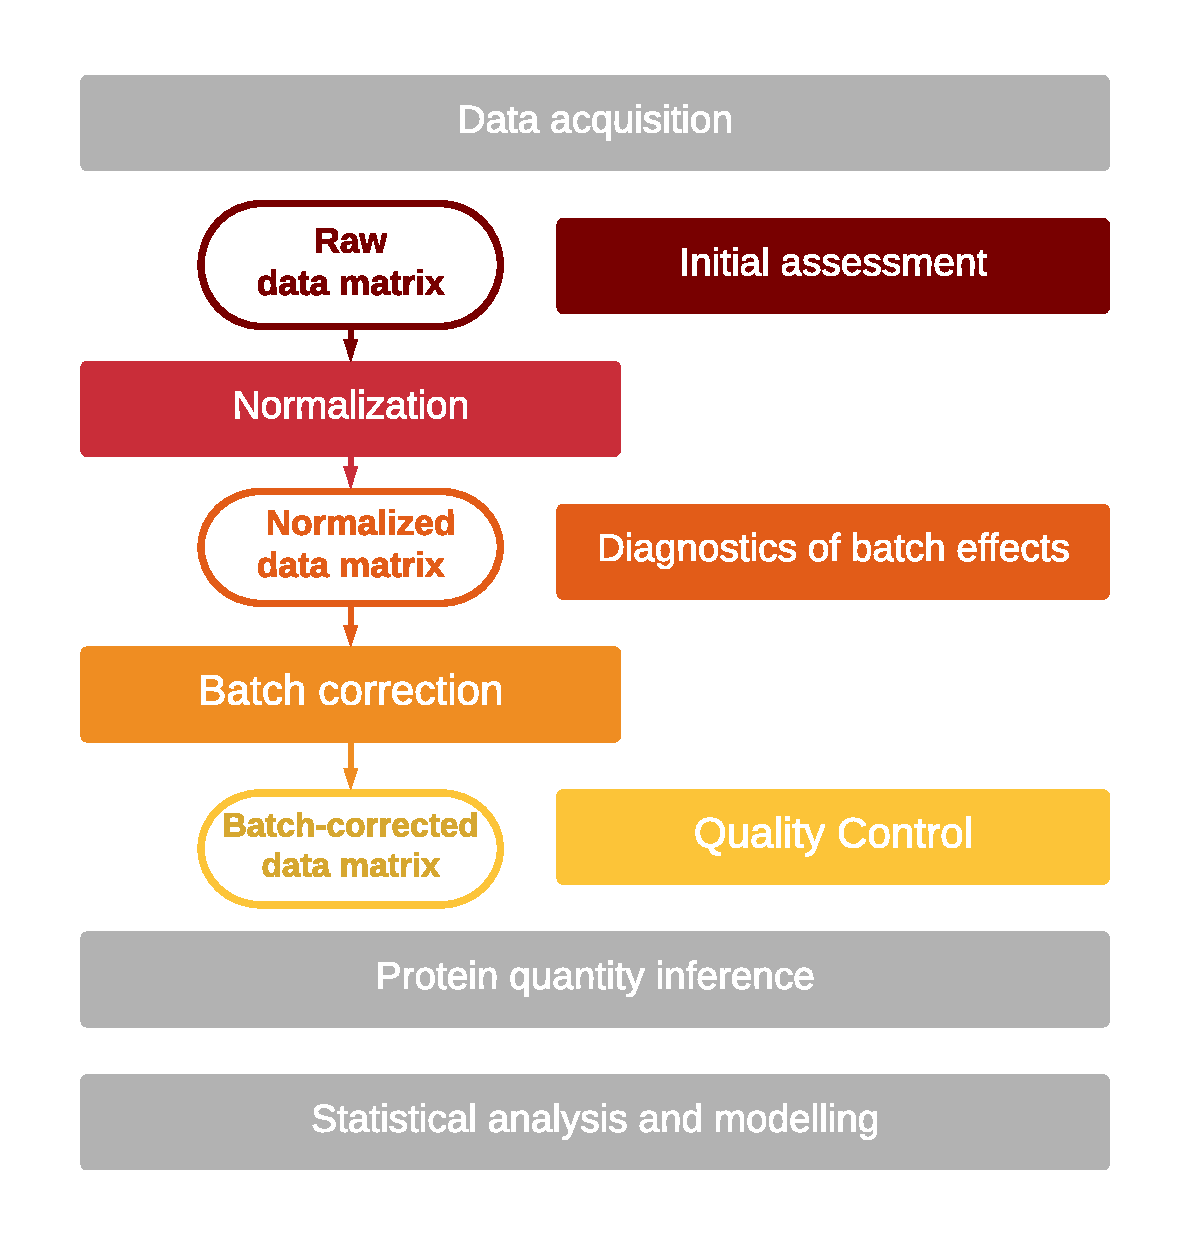
\includegraphics[width=6cm]{figures/Fig0_workflow_staircase}
	\caption[Batch effect correction workflow]
	{\textbf{Batch effect processing workflow}}
	\label{fig:batch_fig1_workflow}
\end{figure}

%We suggest a five-step workflow to address batch effects in large-scale dataset. Initial assessment allows to evaluate whether batch effects are present in raw, unnormalized data and to select normalization procedure. Second, normalization brings all samples from the dataset to the common scale, typical methods of normalization being sample-wide quantile normalization and median normalization. Third step is diagnostics of batch effects in normalized data, with methods such as PCA, hierarchical clustering. This step determines whether further correction is required. If batch effects are still present in the data, a furter step of batch correction is required. Batch correction addresses feature-specific biases, commonly addresses with tools like ComBat \cite{Johnson:2007aa} or feature-specific mean/median centering. Finally, quality control ensures that the data has been improved by correction: biases have been reduces while meaningful signal has been retained. In the next sections, we discuss each step of the workflow in more detail, illustrating it with examples from three large-scale proteomic datasets.

\subsection{Data matrix before adjustment}


This workflow starts with a raw data matrix, for which initial steps, such as peptide-spectrum matching, quantification, and FDR control have been completed. Data are assumed to be log-transformed, unless the variance stabilizing transformation \cite{Durbin2002} is used. In latter case, the data transformation is included into the normalization procedure. 

We strongly suggest to perform batch affect adjustment on peptide or fragment ion level, as this procedure alters feature abundances that are critical for protein quantity inference \cite{Clough:2012aa, Teo:2015aa}.  


We also suggest that all detected peptides, including non-proteotypic and ones with missed cleavages, should be kept into consideration during batch effects adjustment. Keeping all measurements allows to better evaluate the intensity distribution within each sample, which is critical for subsequent normalization and correction steps.

\subsection{Initial assessment}
The goals of the initial assessment phase are to determine bias magnitude, sources and selection of a normalization method.

In most cases, the intensity distributions of samples are different from each other. Comparing global quantitative properties such as sample medians or standard deviations helps with the choice of normalization methods and the identification of technical factors requiring further control. 

Three approaches are particularly useful for initial assessment: 1) plotting the sample intensity average or median, in order of MS measurement or technical batch, allows to estimate MS drift or discrete bias in each batch; 2) boxplots allow to assess sample variance and outliers; 3) Inter- vs. intra-batch sample correlation. A higher correlation of samples from the same batch over unrelated ones is a clear sign of bias.

\begin{table}[hbt]
	\begin{tcolorbox}
		\section*{Box 2: Batch effects processing checklist}
		\label{box:Box2_checklist}
		\begin{tabular}{>{\raggedright}p{2cm}m{10.5cm}}
			\headrow
			\thead{Step} & \thead{Substeps} \\
				
			Experimental design (highlights)	& \begin{enumerate}
				
				\item Randomize samples in a balanced manner to prevent confounding of biological factors with batches (technical factors).
				\item Consider adding replicates
				\item Record all technical factors, both plannable and occurring unexpectedly 
			\end{enumerate} \\ 
			Initial assessment	& \begin{enumerate}
				
				\item Check whether the sample intensity distributions are consistent. 
				\item Check the correlation of all sample pairs
				\item If intensities or sample correlation differ, check whether the intensities show batch-specific biases
			\end{enumerate} \\
		
			Normalization		& \begin{enumerate}
				
				\item Choose normalization procedure, appropriate for biological background and data properties;
				\item \textbf{(!)} If the goal is to determine differentially expressed proteins, and the batch effects are discrete or linear, multi-factor ANOVA on normalized data is a sound statistical approach, as it adjusts for batch effects simultaneously with identification of proteins, that are statistically significant in terms of differential expression. This is true even if diagnostic tools indicate the presence of batch effects.

			\end{enumerate} \\ 
			Diagnostics		& \begin{enumerate}
				
				\item Using diagnostic tools (See \hyperref[box:Box1_definitions]{Box 1}), determine, whether batch effects persist in the data. 
				\item Use quality control already at this step and skip the correction if it is not necessary. 
				
			\end{enumerate} \\ 
			Batch effects correction	& 	\begin{enumerate}
				\item	Choose batch effects correction procedure, appropriate for the biological background and data properties, especially those detected at the previous step.
			\item	Repeat the diagnostic step.
			\item	Assess the ultimate benefit with quality control.
\end{enumerate} \\ 

			Quality control 	& 	\begin{enumerate}
				
				\item	Compare correlation of samples within and between the batches. Pay special attention to replicate correlation, if these are available;
				\item	Compare correlation of peptides within and between the proteins.	
			\end{enumerate} \\ 
		\end{tabular}
		
	\end{tcolorbox}
\end{table}
\clearpage

 



\subsection{Normalization}

The goal of normalization is to bring all samples to the same scale to make them comparable. Two main considerations drive the choice of normalization method: 

\begin{itemize}
    \item \textbf{Heterogeneity of the data: }if samples are fairly similar, the bulk of the proteome does not change and thus techniques such as quantile normalization \cite{Bolstad2003} can be used. In datasets that are dramatically different (i.e. when a large fraction of the variables are either positively or negatively affected by the treatment) different methods, such as HMM-assisted normalization can be used \cite{Landfors2011}. Additionally, if some samples are expected to have informative outliers (e.g. muscle tissue, in which a handful of proteins are several orders of magnitude more abundant then the rest of the proteome), methods that keep the relationship of outliers to the bulk proteome, need to be used \cite{Wang770115}.

    \item \textbf{Distribution of sample intensities: }The initial assessment step, especially boxplots, indicate, which level of correction is required: in most cases, shifting the means or medians is enough, but when variances differ substantially, these need to be brought to the same scale as well.
\end{itemize}
It should be noted, that after normalization no further data correction might be required. This can be determined with the diagnostic plots and quality control methods, described below. If the results are satisfactory, keeping data manipulation minimal is always advisable.

\subsection{Diagnostics of normalized data}

While normalization makes the samples more comparable it only aligns their global patterns. Therefore, batch effects affecting specific proteins or protein groups might still represent a major source of variance even after normalization. Thus, diagnostic of batch effects is most informative when performed on the normalized data. 

The diagnostic approaches can be divided in proteome-wide and peptide-level approaches. The main approaches for \textbf{proteome-wide diagnostics} are:
\begin{itemize}
	\item \textbf{Hierarchical clustering} is an algorithm that groups similar samples into a tree-like structure called dendrogram. Similar samples cluster together and the driving cause of this similarity can be visualized by coloring the leaves of the dendrogram by technical and biological factors. Hierarchical clustering is often combined with a heatmap, mapping quantitative values in the data matrix to colors, which in turn facilitates the assessment of patterns in the dataset.
	\item \textbf{Principal Component Analysis (PCA)} is a technique that identifies the leading directions of variation, known as principal components. The projection of data on two components allows to visualize sample proximity. This technique is particularly convenient to assess clustering by biological and technical factors, or to check replicate similarity (works well until about 50-100 sample in a dataset). 
	\item \textbf{Principal Variance Component Analysis (PVCA)}. PVCA maps each principal component to technical and biological factors, assessing the weight of each factor in each component. These weights are then combined with the variance fraction of each component, thus quantifying the variance, associated with each factor, both technical and biological. Thus, PVCA turns the intuition of PCA into a quantitative readout. 
\end{itemize}

One should be careful, however, in interpreting proteome-wide diagnostics, as all of them were designed for data matrices without missing values. For more details, we refer the reader to %\ref{Box_3_Missing_values}.

In proteomics \textbf{peptide-level diagnostics} are as useful as proteome-wide diagnostic. As in other high-throughput measurements, individual features, in this case peptides, are visualized to check for batch-related bias. In proteomic datasets, spike-in proteins or peptides can be added as controls and used for this purpose. In most DIA datasets  iRT peptides \cite{Escher:2012aa}, if added in precise concentrations, are very well suited for individual feature diagnostics.
It should be noted, however, that any random peptide should not be biased in a batch-related manner, so checking a handful of endogenous peptides can also be informative.

Another reason to check individual peptides in proteomics is to examine the trends associated with sample running order. These trends might occur as MS signal deteriorates and require special correction approaches.

\subsection{Batch effects correction}

Diagnostics helps to determine, whether batch effects correction is needed. As global sample patterns have already been corrected during normalization, batch effects affect specific features and feature groups, and that’s the level on which they need to be corrected.

If batch effects are continuous, i.e. manifest as MS signal drift, an order-specific curve needs to be fitted. Such drifts are more likely to occur in studies profiling hundreds of samples. Since this is a problem that is specific to mass spectrometry and is still relatively new for the community, we propose a solutions for it in  \ref{Box_4} Box 4 “Correcting MS signal drift”.

More commonly batch effects are discrete and manifest as feature-specific shifts of each batch. For these cases, methods such as mean and median centering work very well. A more advanced modification of the mean shift is provided by ComBat \cite{Johnson:2007aa}, that uses a Bayesian framework, which has been successfully applied to proteomic data \cite{Lee:2019aa}. However, this requires that all features are represented in each of the batches. Therefore, especially in large-scale proteomic datasets, applying ComBat might require removal of  a prohibitively high number of peptides,  (see \hyperref[box:Box3_missingness]{Box 3 “Missing values”} for details).

\subsection{Quality Control}

The purpose of the quality control step is to determine whether the adjustment procedures – normalization and/or batch effects correction – have improved the data. At this step, the data after adjustment are compared to the raw data matrix.

There are two types of criteria to evaluate the data quality: 1) Removal of the bias (negative control); 2) Improvement of the data (positive control).


Typically, bias is considered to be removed, if diagnostic plots indicate that similarity between samples is not driven by technical factors anymore. This means that neither hierarchical clustering nor PCA show clustering by batch, and correlation of samples from the same batch is no longer stronger than correlation of unrelated samples. Also, individual features should not show batch-related biases. Thus, comparison of diagnostic plots for raw and adjusted data serves as the negative control.

Proving the improvement is, however, much harder. It is common to take “improved clustering by biological condition” or “higher number of differentially expressed proteins” as a positive control and generally, as a sign of data quality improvement. However, both criteria can be subjective: it is impossible to know beforehand, whether biological groups are separable in the proteomic space, especially if only a subset of proteins changes and the bulk of the proteome is not. Similarly, it is not possible to predict, whether higher sensitivity for differential expression comes at the expense of added false positive hits. Therefore, we do not recommend these criteria for the assessment of the method of normalization or batch effects correction: the choice of the method should rather be based on properties of the samples as described above. However, since batch adjustment removes a certain portion of variance, the coefficient of variation for peptides and proteins in replicated samples should decrease. This is especially true for spike-in peptides or protein that are added to samples in controlled quantities. 

A stronger positive control is assessment of reproducibility. More precisely, one can compare lists of differentially expressed proteins or predictive performance of regression/classification models derived from two or more sample sets belonging to different batches \cite{Lazar:2013aa}. It is expected that in adjusted datasets, the resulting lists of differentially expressed proteins, or proteins providing optimal class separation, will be highly overlapping \cite{Shabalin:2008aa}. If two sample sets are independently used for predictive modeling, the predictive performance of such models is also expected to be comparable in adjusted datasets \cite{Luo2010}. Note however, that while this method generalizes well to studies with data acquired by different technologies (e.g. microarrays and RNA-seq for transcriptomics or DIA vs TMT for proteomics), it is restricted to fairly large datasets, as predictions from small-scale experiments tend to be unstable.
 
Here we also propose two positive control methods, that do not rely on large sample size and are applicable to most proteomic experiments. The first is based on sample correlation. It is expected, that the correlation of replicate samples  is higher than the correlation of unrelated samples. Particularly, the distribution of replicate correlations should be clearly shifted upwards, even though replicates might occasionally correlate less well than some unrelated sample pairs, and this distinction should be strengthened by batch adjustment procedures. The second assessment method is specific for bottom-up proteomics, and makes use of peptide correlation. Correlation of unrelated peptides is expected to be close to zero, while peptides originating from the same protein are likely to be positively correlated. Since tens of thousands of peptides are routinely detected in a modern high-throughput proteomic experiment improvements in this metric are a reliable readout of data quality following batch adjustment.

\section{Datasets description}\label{subsec:datasets}

To illustrate the application of the workflow described above, we use two published and one unpublished large-scale proteomic datasets, described in the Table~\ref{tab:batch_datasets}. 

The first study, called here \textbf{"InterLab study"}, assessed the robustness of SWATH-MS in a multi-lab setting \cite{Collins2017}. A set of 30 stable isotope labeled standard (SIS) peptides \cite{Ebhardt2012}, partitioned in five groups, was serially diluted in HEK293 cell lysate. The SIS peptides in the resulting samples spanned a concentration range from 12 amol to 10 pmol. These five samples sets were distributed to 11 laboratories worldwide for measurement by SWATH-MS according to a predetermined schedule. Each of the samples was run on 3 separate days, with the exception of the 4th sample that was run three times on each day. In total, 229 samples were profiled. Thus, the technical covariates whose effect needed to be assessed were the data acquisition site and day. Note that due to the technical nature of the study no biological signal needed to be identified. As only a small number of SIS peptides is different across these samples, all changes can be attributed to technical covariates and therefore the samples in this study can be treated as replicates. Within this manuscript, we analyze only the influence of the acquisition site as a batch factor.

The second study, named here \textbf{"PanCancer study"} \cite{Sajic2018}, profiled the blood proteome of a cohort of patients with five solid carcinomas and matched controls. In total 155 blood plasma samples were collected. Protein digestion and glycopeptide enrichment were performed in 4 batches, several weeks apart. To control for measurement reproducibility, 7 biospecimens were replicated and allocated to a different batch. To control for intra-sample variation caused by the sample preparation protocol, bovine fetuin-B was spiked in equal amounts into each plasma sample.

The third dataset called here \textbf{"Aging mouse study"}, has not yet been published. In this study, the liver proteomes from a BXD reference mouse population \cite{Peirce:2004aa} were profiled to identify proteome changes associated with age. Similarly to prior BXD mice metabolic profiling experiments \cite{Williams:2016aa} the animals were also subjected to Chow or High-Fat Diet. The samples were randomized with respect to biological covariates (age, diet, sex) and two mice samples with EarTags "ET1506" and "ET1524" were measured every 10-15 MS runs to control for signal consistency. Overall, the samples were digested in four batches. To compensate for signal deterioration, MS data acquisition was interrupted for machine cleaning and tuning six times, resulting in 7 mass-spectrometry batches. Additionally, these were mostly confounded with digestion batches. To allow for better evaluation of the mass-spectrometry batch effect, 10 samples profiled at the end of batch 3, were profiled again after each machine tuning. In total, 375 samples were analyzed. \textcolor{blue}{Details about the experimental condition and proteomic profiling can be found below in section \ref{sec:mouseProteome}. \textbf{SHALL WE KEEP THIS SENTENCE and add the experimental details?}}

All in all, these datasets are representative of various applications of large-scale proteomic studies. They make use of various sample sources (i.e. cell cultures, patients and mice). They ask technical and biological questions in proteomes of varying complexity. They present different degrees of sample-to-sample heterogeneity. In this respect, the InterLab study is very homogeneous, to the point that its samples are essentially technical replicates. The PanCancer study is highly heterogeneous, since as little as 295 proteins were identified in samples originating from different hospitals and cancer localizations. Finally, the Aging mouse study represent an intermediate case. On one hand, its subjects were genetically very similar and were grown in a controlled environment. On the other hand, sampling from tissues introduced a certain amount of heterogeneity.

\begin{landscape}
	\begin{table}
		\renewcommand*{\arraystretch}{1.8}
		\caption[Dataset description]{Dataset description. For aging study: number of proteins and peptides before filtering for completeness}
		\label{tab:batch_datasets}
		\small
		\begin{tabular}{|  m{1.75cm}|  m{1.15cm} |  >{\raggedright}m{1.5cm} | >{\raggedright}m{4.13cm} |  m{2.5cm} |  >{\raggedright}m{2.2cm} |  m{1.5cm} |  m{1.5cm} |}
			\hline
			\textbf{Sample} & \textbf{Organism} & \textbf{Sample source} & \textbf{Sample-to-sample heterogeneity} & \textbf{Technical factors} & \textbf{Biological factors} & \textbf{Protein (peak group) number} & \textbf{Number of samples} \\
			\hline
			\hline
			\textbf{InterLab study} & human & cell culture & very low: 
			samples come from the same tissue cultures and differ only by few spike-in peptides
			& \vspace*{1em}\squishlist
			\item data acquisition sites
			\item profiling days
			\squishend
			& --- & 4077
			(31886)
			& 229  \\
			\hline
			\textbf{PanCancer study} & human & blood & high: 
			samples come from cancer patients and matched controls with different cancer localization
			& \squishlist
			\item protein digestion batch
			\squishend
			& \squishlist
			\item case / control
			\item cancer localization
			\squishend
			& 203 (1360)
			& 171  \\
			\hline
			\textbf{Aging mouse study} & mouse & liver tissue & medium: 
			samples come from population of inbred samples originating from two parental strains
			&  \vspace*{1em}\squishlist
			\item protein digestion batch
			\item MS batch
			\item MS drift
			\squishend
			& \squishlist
			\item Strain
			\item Diet
			\item Age
			\squishend
			& 5436*
			(33157*)
			& 371  \\
			\hline
		\end{tabular}
	\end{table}
\end{landscape}

\section{Case Studies}\label{subsec:case_studies}
\subsection{Initial assessment}
The main goal of the initial assessment is to set a baseline for the magnitude and nature of batch effects in a particular dataset. At this stage the data matrix is “raw” in a sense, that the quantities are reported as measured, without any calibration, normalization or correction with regard to the quantities in other samples.


\begin{figure}[hbt]
	%\center
	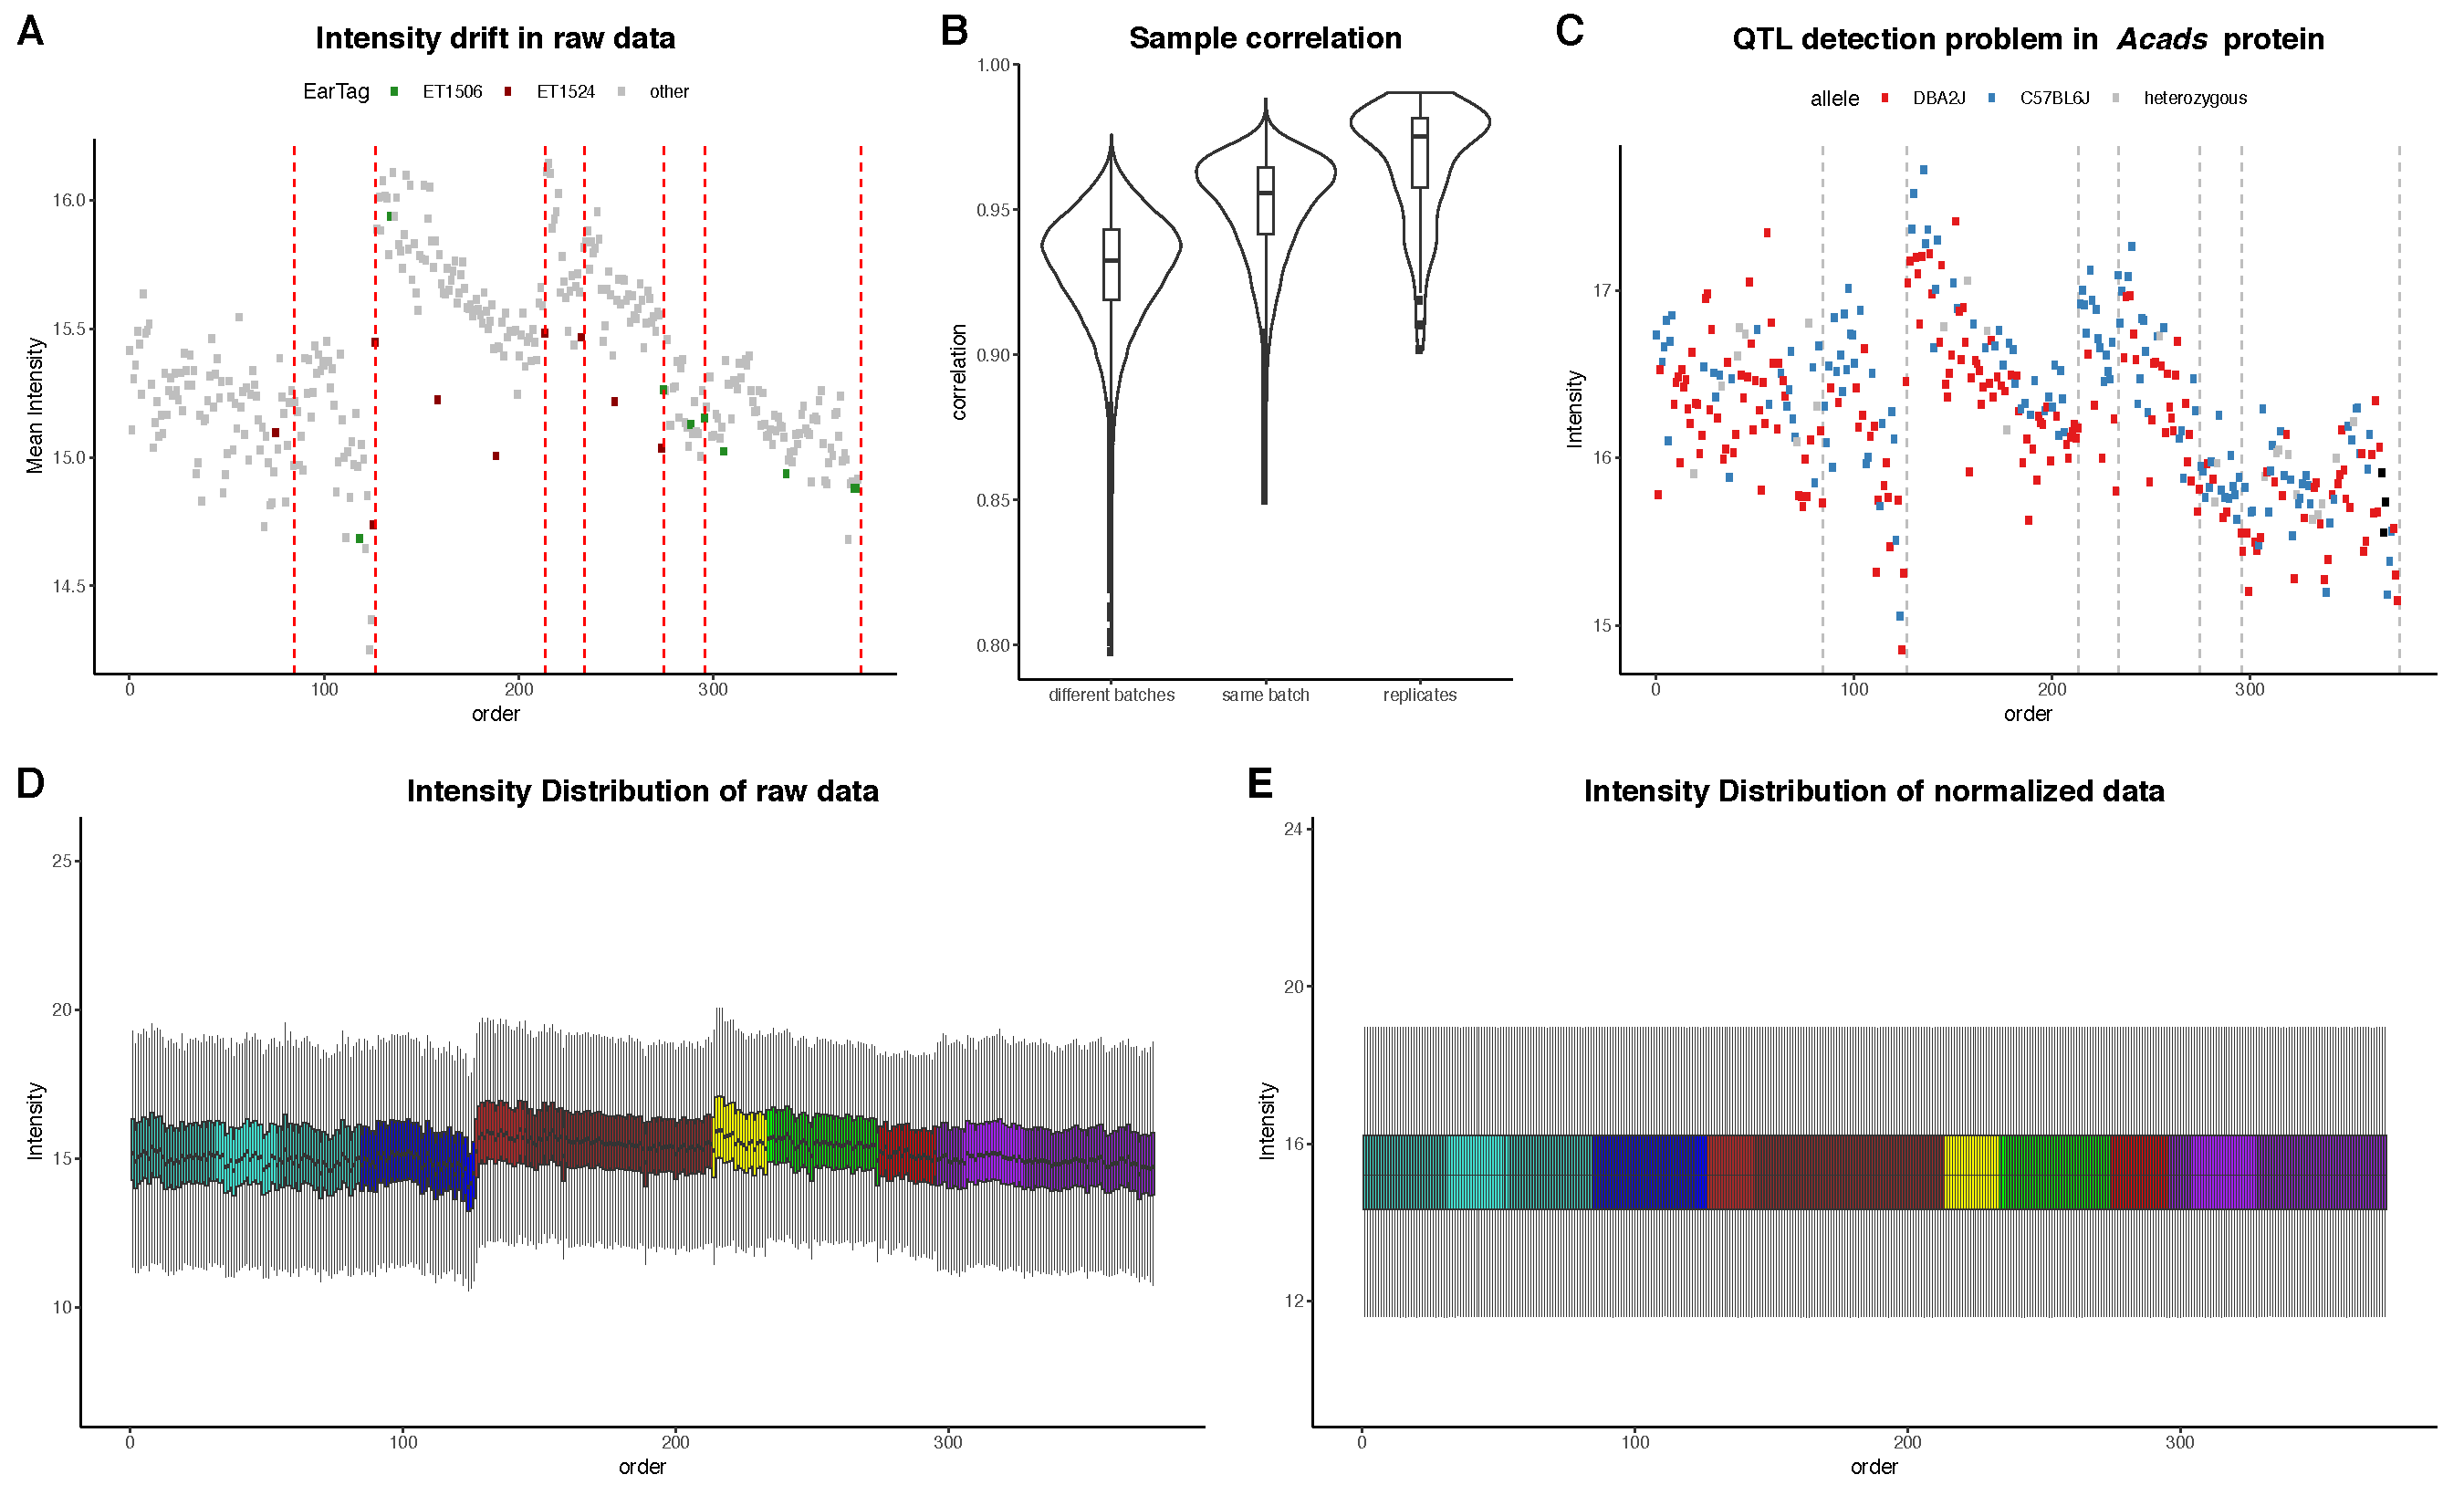
\includegraphics[width=\textwidth]{figures/Fig1_initial_assessment_v5_edited.pdf}
	
	\caption{\textbf{Initial assessment and normalization of the Aging mouse study} \\
		\footnotesize
		(A) Mean Intensity in raw data vs sample running order with repeatedly replicated samples shown in color. Vertical dotted lines indicate likely MS-batch boundaries; (B) Distribution of unadjusted sample intensity correlations - between batches, within batches and in replicated samples; (C) Representative "Acads" protein QTL, that cannot be detected due to the signal drift; (D) Boxplots of sample intensities in raw, unnormalized data; (E) Boxplots of sample intensities after normalization}
	\label{fig:batch_fig2_initAssessment}
\end{figure}

Thus, it is essential to get a quick overview of the data by comparing global statistics, such as average intensity or correlation of samples, and few individual proteins, for which there is some prior information on their expected abundance. In mass-spectrometry, it is important to plot these statistics in a sample running order, as it is not uncommon for the measured signal to start drifting. This is clearly seen on Figure~\ref{fig:batch_fig2_initAssessment}A, where the average intensities of samples from the Aging mouse study are plotted vs the sample running order. In this case, the intensity tended to deteriorate after 50-70 samples. The resulting interruptions for cleaning and calibrating of the instrument determined the mass-spectrometry batch. As this type of bias cannot be entirely planned for in advance, it is particularly important to randomize the samples and to include replicates (for more details on sample replication in this dataset see Section~\ref{subsec:datasets}“Dataset description”). 

Not only do batch effects introduce shifts in the total sample intensity distributions, but they also lead to spurious correlation between features (i.e. fragments, peptides or proteins). It is common, for samples belonging to the same batch to have strong correlation (as seen in Figure~\ref{fig:batch_fig2_initAssessment}B, Figure~\ref{fig:batch_figS1_InterLab}B). Often this correlation is not only stronger than the correlation of samples from different batches (“between batches”), but also stronger than the correlation of replicates. Hence, the importance of assessing correlation distributions as early as possible. Sample correlation can be visualized as a clustertmap (InterLab Study, Figure~\ref{fig:batch_figS1_InterLab}B) or as a correlation distribution box/violinplot (Figure~\ref{fig:batch_fig2_initAssessment}B). The former is preferred with smaller sample sizes (i.e. roughly < 150 samples) and the latter with large datasets.

Optionally, one can complement the initial assessment with the analysis of a few specific features (peptides or proteins), for which prior information is known. In our case, we plotted several proteins with known quantitative trait loci (QTL). However, as seen in Figure~\ref{fig:batch_fig2_initAssessment}C, the intensity drift prevented the corresponding alleles from being separated.

Last but not least intensity boxplots are extremely powerful at this stage of the analysis, as they visualize in a single plot median, quantiles and outliers. This allows one to see, whether there are batch-specific intensity patterns such as shifts (as in the InterLab study, see Figure~\ref{fig:batch_figS1_InterLab}A), or drifts (as in Figure~\ref{fig:batch_fig2_initAssessment}D), or no evident batch-associated patterns (PanCancer data, Figure~\ref{fig:batch_figS2_PanCancer}A). To detect the patterns, the samples should be sorted by running order or by batch (if the batches, such as digestion batches have been randomized prior to MS analysis). Note that in some cases, intensity patterns might be easier to spot on average intensity plot (compare to Figure~\ref{fig:batch_fig2_initAssessment}A).

\subsection{Normalization}

Normalization is an essential step in removing bias from the data as it brings the samples to the same scale, making the measured quantities comparable. As stated in “protocol overview”, the choice of normalization should take two factors into account: 1. heterogeneity, as assessed from previous knowledge, and; 2. global quantitative sample properties, e.g. mean/median/variance, as indicated by initial assessment.

The most common type of normalization, quantile normalization \cite{Bolstad2003}, is applicable to wide a range of samples and was chosen for the Aging mouse data and the PanCancer dataset. As shown in Figure~\ref{fig:batch_fig2_initAssessment}D and E (and Figure~\ref{fig:batch_figS2_PanCancer}A and B), the intensity distributions after quantile normalization are very similar.  This is desirable in experiments where the majority of features are not expected to change, but can be problematic in experimental setups where outliers bear important information.

Median centering normalization only brings the medians to the same scale and thus is a “milder” approach. This normalization was chosen for the InterLab study and brought the peptide quantities measured at different sites much closer to each other (see Figure~\ref{fig:batch_figS1_InterLab}C). In this dataset, shifting the medians to the same value (see Figure~\ref{fig:batch_figS1_InterLab}D) was sufficient do remove a substantial portion of bias. The resulting improvement in signal quality is also reflected in the improved protein quantification precision as illustrated by the reduction in  coefficient of variation for the majority of proteins in the dataset (see Figure~\ref{fig:batch_figS1_InterLab}E).

As shown in this example normalization alone is sometimes the only required correction. In the median normalized InterLab study, the improvement of quantification of spike-in peptides (Figure~\ref{fig:batch_figS1_InterLab}C) and the decrease in protein coefficient of variation (Figure~\ref{fig:batch_figS1_InterLab}E) serve as quality control, and indicate that the further batch correction steps can be skipped.

This of course not always the case, and batch effects diagnostics should be used, as presented in the next section, to determine if further correction steps are required.


\subsection{Diagnostics}

\begin{figure}[hbt]
	%\center
	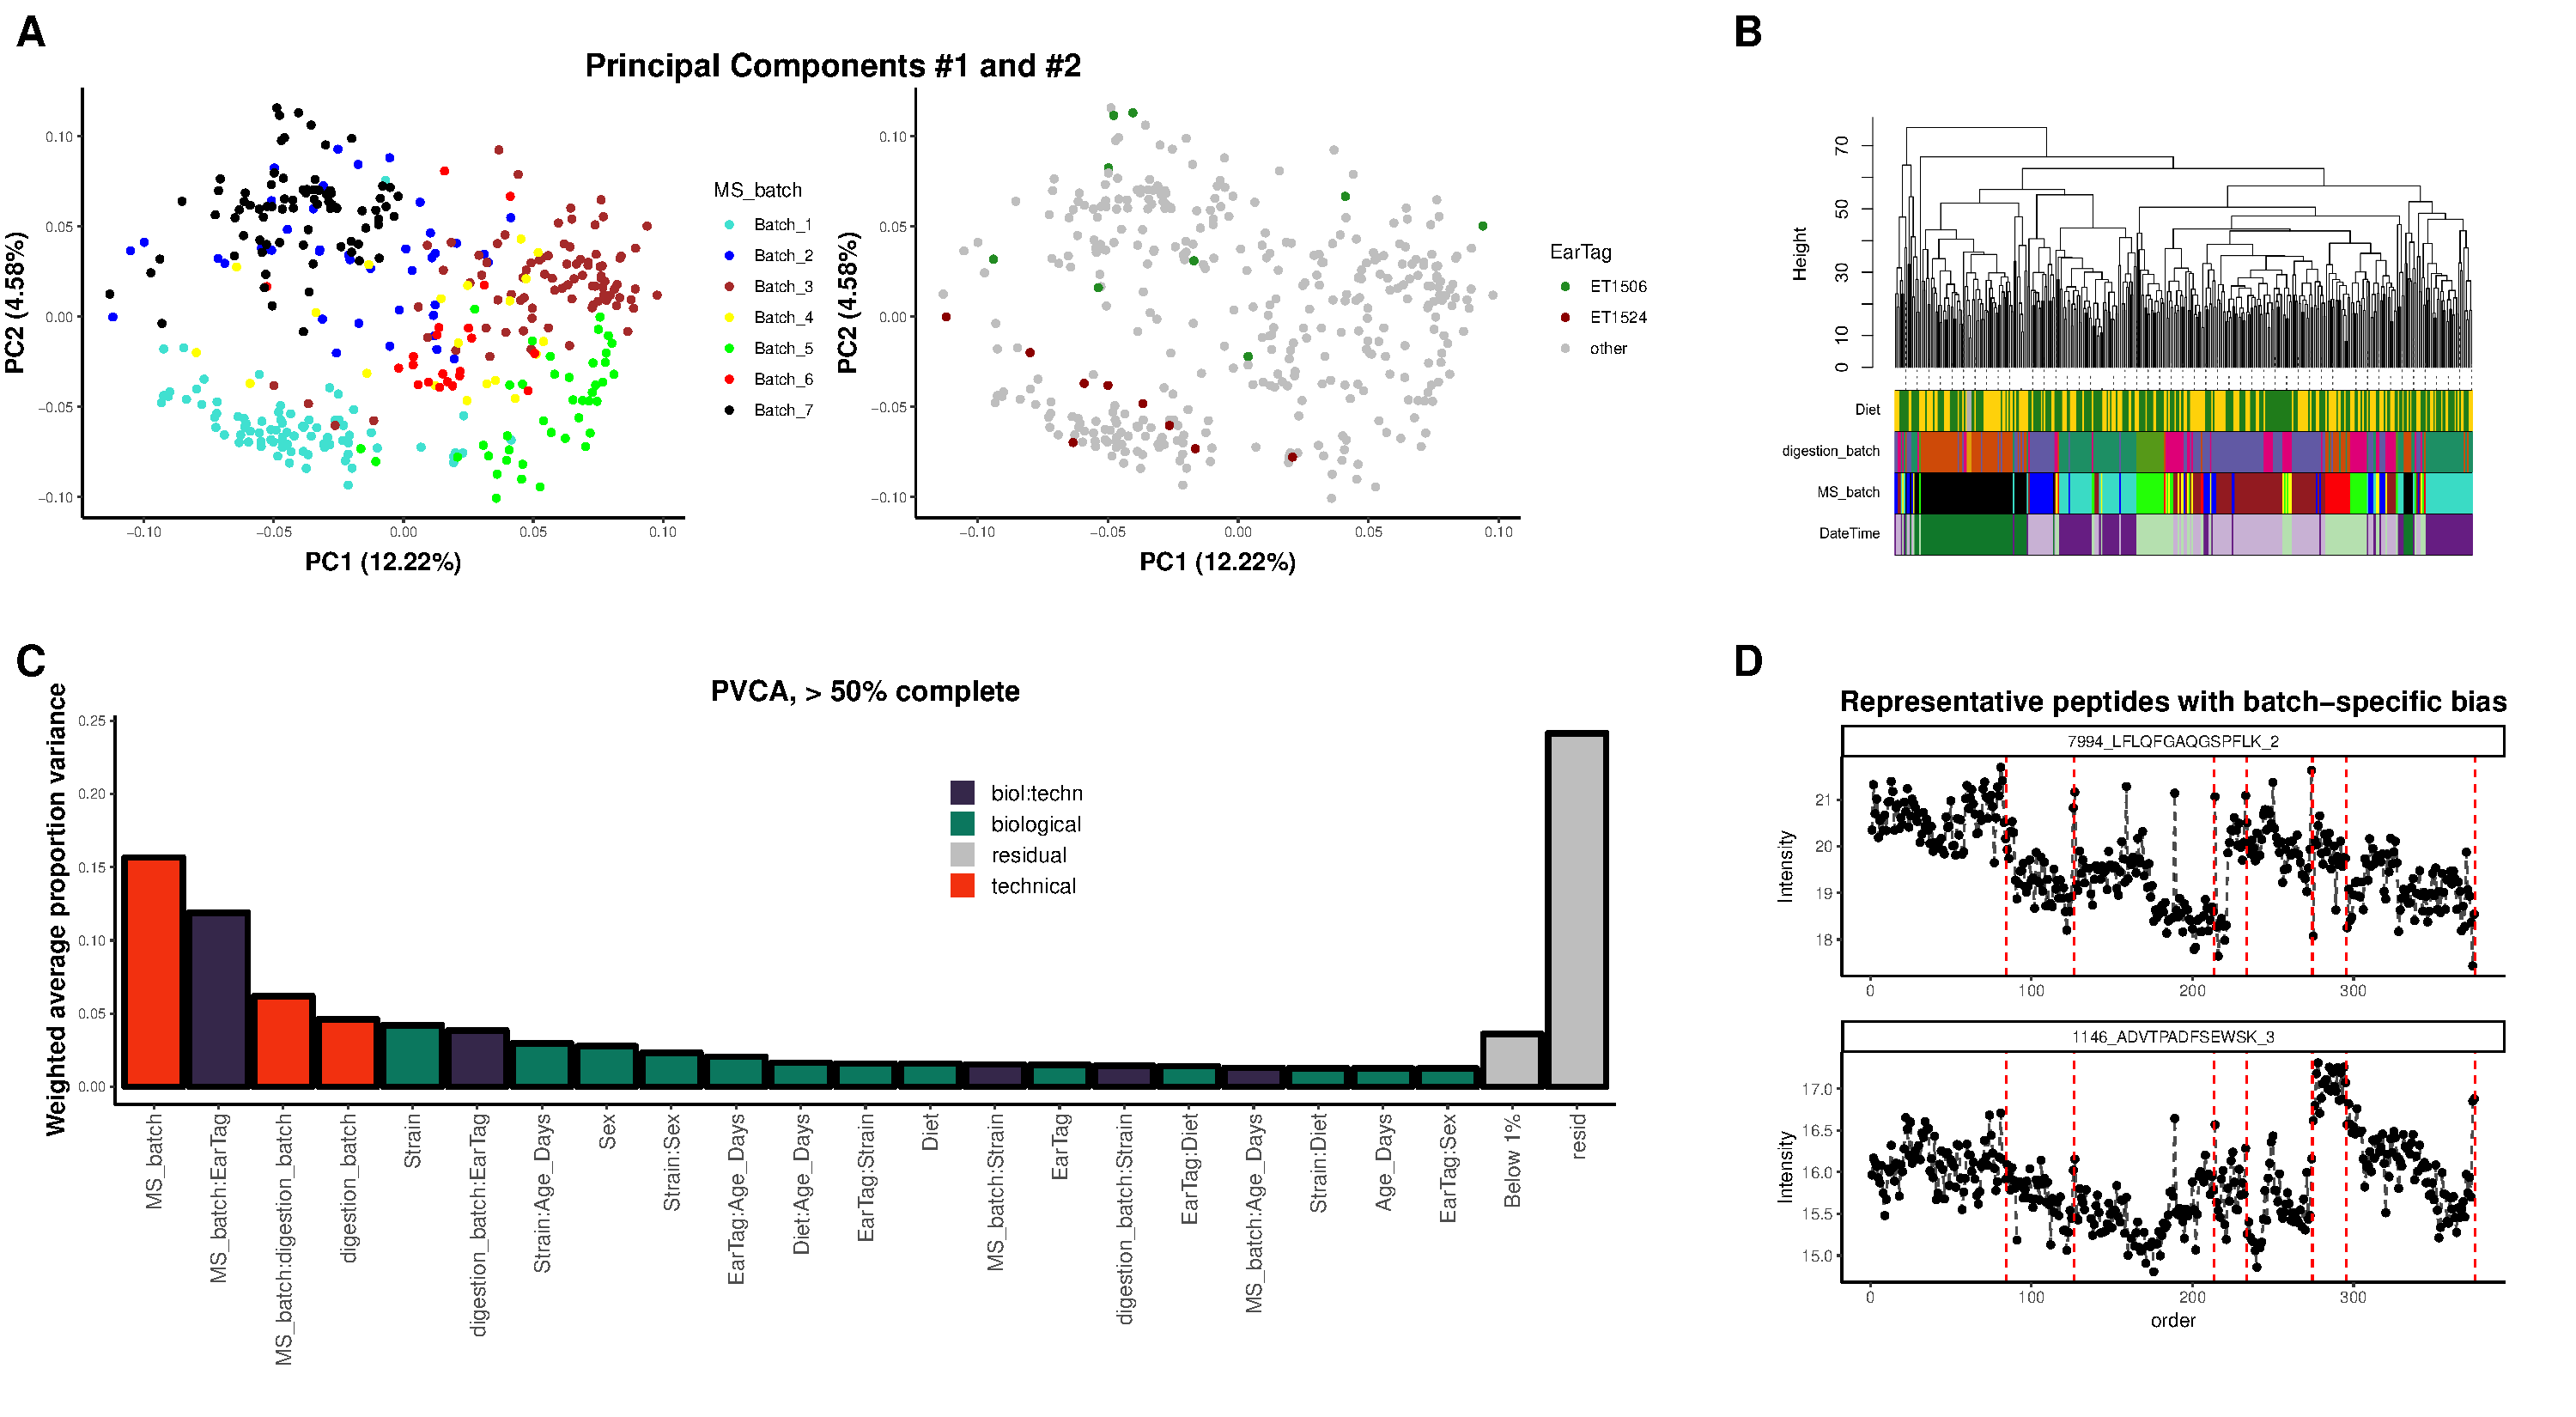
\includegraphics[width=\textwidth]{figures/Fig2_diagnostics.pdf}
	
	\caption{\textbf{Diagnostics of batch effects}  \\
		\footnotesize
		(A) Principal Components \#1 and \#2 colored by MS batch (left) and replicates (right). The effect of clustering by MS- batch is dominating, but the replicated samples are closer to each other than just random samples; (B) Hierarchical clustering of samples, with leaves colored by Diet, digestion batch, MS batch and Date-time of sample acquisition is dominated by technical factors; (C) Principal Variance Component Analysis of peptides, detected in >50\% of samples demonstrates, that the technical factors, such as MS batch, digestion batch and their combination has a profound effect on the data, while biological factors such as Strain, Sex and Age account for a much smaller fraction of variance; (D) Peptide-level plots for two iRT peptides demonstrate, that batch effect manifests also as MS signal drift that requires correction}
	\label{fig:batch_fig3_diagnostics}
\end{figure}

Normalization harmonizes overall sample intensities, however, batch effects can still be present at the level of specific features and bias the quantities of many peptides and proteins.
Various methods can be used to assess the extent of bias in the data. Most of them characterize the dataset as a whole, thus working on proteome level. Methods like Principal Components Analysis (PCA) and Hierarchical Clustering are the most established. They allow to visualize the factors underlying the similarity of the samples.
Principal Component Analysis is a method that transforms the data matrix into a linear combination of “components” representing the directions of highest variance in the data. This allows high-dimensional data to be visualized in lower dimensions. Additional coloring of the samples by technical/biological factors or by highlighting replicates facilitate the interpretation of what drives sample proximity. For instance, in the Aging mouse study, the following patterns become apparent (see Figure~\ref{fig:batch_fig3_diagnostics}A): first, we see a strong clustering of samples by mass spectrometry batch; second, while replicates tend to be close, they are not necessarily the samples with the smallest distance to each other. An overlaid visualization of other factors, such as digestion batch, diet or acquisition date can be found in \textcolor{red}{Supplementary Fig3A}.
 
Hierarchical clustering in contrast, allows one to visualize multiple factors at once (Figure~\ref{fig:batch_fig3_diagnostics}B). Overall, the same patterns identified in the PCA plots are confirmed: clustering is driven primarily by MS and digestion batch, while the effect of diet, the biological factor, is not as strong. Similarly, in the PanCancer study (Figure \ref{fig:batch_figS2_PanCancer} {top parts of E and F}), we see that the digestion batch is the key clustring factor.

Principal Variance Components Analysis (PVCA) transforms the intuition of visualization brought about by PCA and Hierarchical Clustering into numbers. The weights of each factor in each Principal Component are combined, thus providing a concise summary of variance distribution between biological and technical factors and their combination. In the Aging mouse dataset we see in Figure~\ref{fig:batch_fig3_diagnostics}C, that technical factors such as MS batch, digestion batch and their combination are leading drivers of variance. Whereas biological factors, such as Diet, Sex and Age are much less prominent. It should be noted, that a substantial fraction of variance is “residual”, and cannot be explained by the annotated sample characteristics.

It is important to point out, that most proteome-wide diagnostics rely on data matrices without missing values. Typically for PCA or hierarchal clustering the missing values are imputed (e.g. filled with zeros, small random numbers, ...). However, since missing values are often batch-specific, this might lead to an overestimate of the batch-related clustering. For more details on the effect of missing values, please refer to \hyperref[box:Box3_missingness]{Box 3 “Missing values”}.

In addition to proteome-wide diagnostics, it is highly advisable to select a few individual features to assess for the presence of feature-level bias. Spike-in peptides and proteins are particularly handy for this type of diagnostics. We illustrate this in the Aging mouse data using iRT peptides, that were spiked at constant quantities in all samples. In Figure~\ref{fig:batch_fig3_diagnostics}D, one can see, that despite the initial normalization, batch-specific bias still affects the signal. Moreover, this bias is order-related and manifests differently for each of the peptides (for example, in samples \textcolor{red}{125 – 206}). In the PanCancer study, we instead use peptides from the spiked-in Bovine protein Fetuin B. Also in this case, the spike-in peptides are quantified differently in each batch (Figure \ref{fig:batch_figS2_PanCancer} {C}). Contrary to the Aging mouse study here there is no order-related drift, but rather each batch mean is shifted. In conclusion, feature-level bias can be very different in each dataset and checking several representative peptides can help understand the exact nature of the bias.

Together, proteome-level and feature-level diagnostics guide the choice of appropriate batch correction procedure.

\afterpage{%
	\begin{tcolorbox}
		\section*{Box 3: Missing values}
		\label{box:Box3_missingness}
		Proteomics experiments now routinely profiles hundreds or thousands of proteins. However, detecting all proteins without missing values across hundreds of samples is not yet feasible. The patterns of "missingness" are known to be batch-specific \cite{Karpievitch2012}, which is also true for the Aging mouse data (see Figure~\ref{fig:batch_fig4_missing_values} \textcolor{red}{\textbf{\hl{and Supp Fig X}}} for details).
		
		It should be noted, that although "missingness" among low-abundant proteins and peptides is more common, this problem can arise due to peptide interference regardless of their abundance. 
        Missing values can also affect batch effects correction methodologies. For instance the current implementation of ComBat \cite{Johnson:2007aa} does not work if a peptide is missing in one batch. One possible solution is to remove all peptides with missing values before the batch correction \cite{Lee:2019aa}. However, this leads to the loss of potentially valuable quantitative data. Thus, methods which are more robust to missing data, such as median-centering, can sometimes be better suited for proteomic data.
		
		Missing values are often imputed, by filling them with zeros, random small values \cite{Tyanova:2016aa} or re-quantification of elution traces \cite{Rost2016}. Such imputation, however, can introduce bias that is batch- or peptide-specific, as seen in  \textcolor{red}{\textbf{\hl{(Supp Fig Xa)}}}. In turn, this skews batch effect diagnostic methods, such as hierarchical clustering, PCA or PVCA. In these cases, batch effects will be overestimated, as the clustering pattern will be driven by missing values Fig~\ref{fig:batch_fig4_missing_values}A. One can estimate this effect by varying the fraction of missing values and assessing to what extent the batch effects are driven by consistently quantified peptides vs missing ones \textcolor{red}{\textbf{\hl{Supp Fig Xb}}}.
		

		Much more importantly, imputed values may also bias the analysis past the batch effect adjustment stage. As shown in Fig ~\ref{fig:batch_fig4_missing_values}B and C, if "requant" values are used, the correlation within batches seems higher than the correlation of replicates, while this problem is not observed when imputation is not used "no requants".
		
		Finally, provided that there are enough confidently quantified values, many downstream analysis techniques, such as differential expression or protein correlation analyses, can handle missing values. We therefore, advise avoiding imputation, or at least performing it after batch correction whenever possible. 

		
		\begin{minipage}[h]{\linewidth}
			%\center
			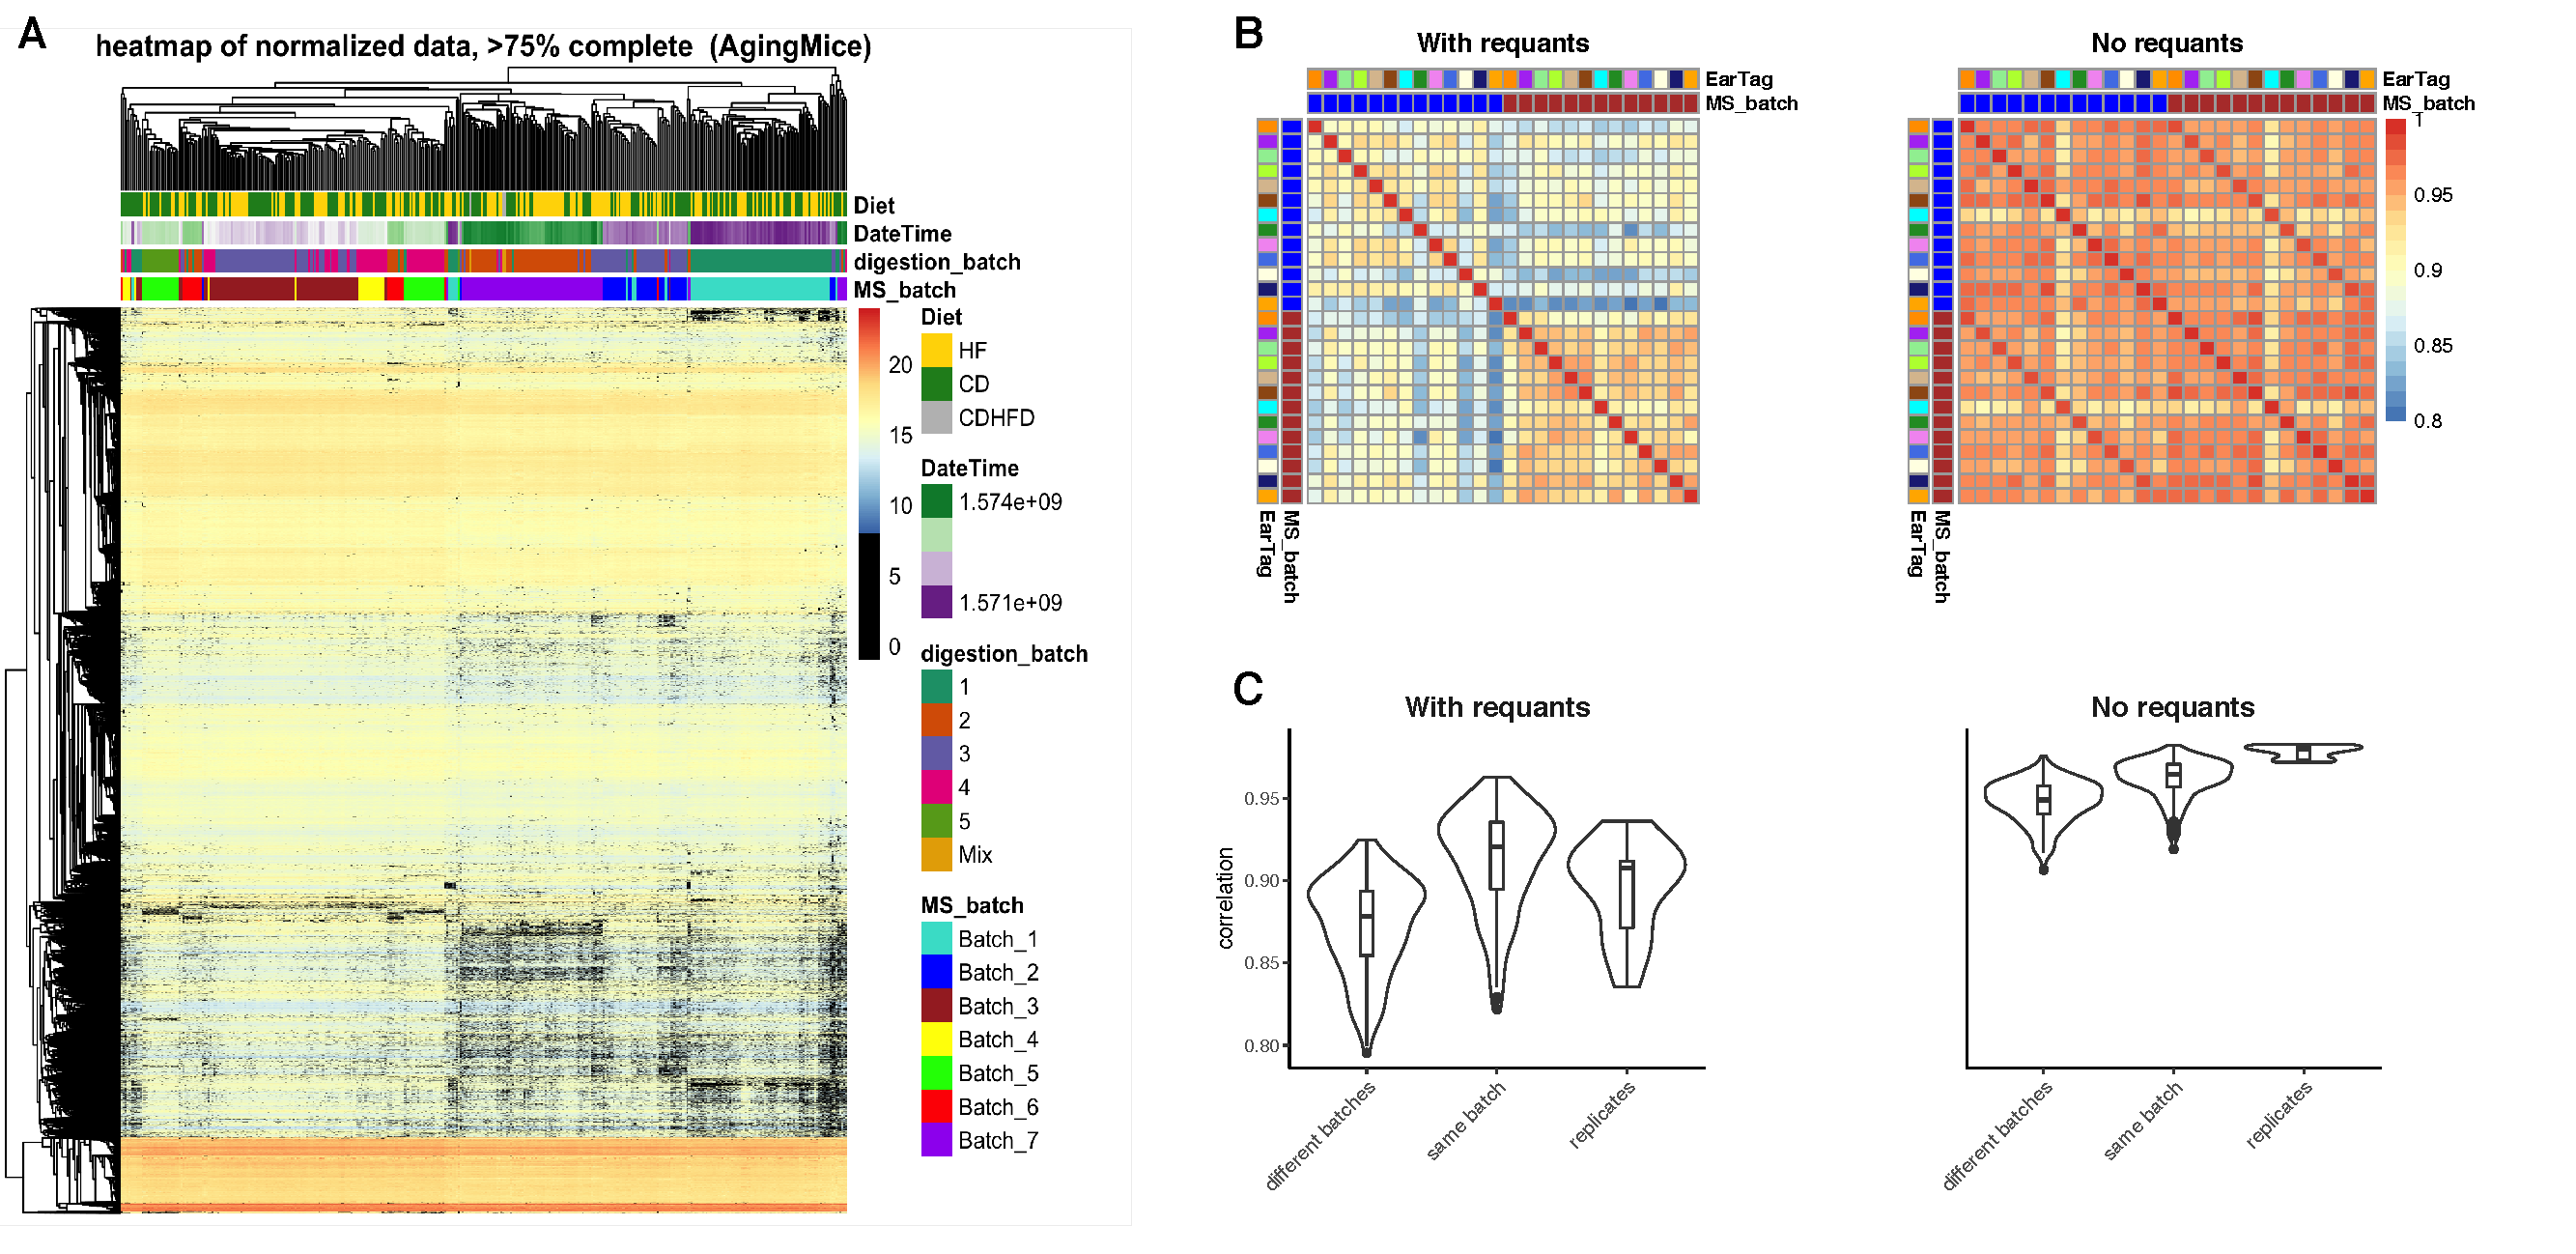
\includegraphics[width=.9\textwidth]{figures/Fig4_missing_values.pdf}
			\captionof{figure}[l]{\textbf{The problem of missing values in batch effect diagnosis and correction} }
			\label{fig:batch_fig4_missing_values}
			{\footnotesize  (A) Hierarchical clustering of normalized data; Missing values are shown in black. The missing values are non-randomly associated with the batch; (B) Heatmap of selected sample correlation: stronger correlation of samples within Batch 2(blue) and Batch 3 (brown) is visible in the data with "requants", and replicate correlation is much more prominent in the data without "requants";	(C) Distribution of selected sample correlation: same effect, as in (B) is shown with violin plots of sample correlation. All data from the Aging mouse study.}
		\end{minipage}
	\end{tcolorbox}
	\clearpage
}


\subsection{Batch effects correction}
\begin{figure}[hbt]
	%\center
	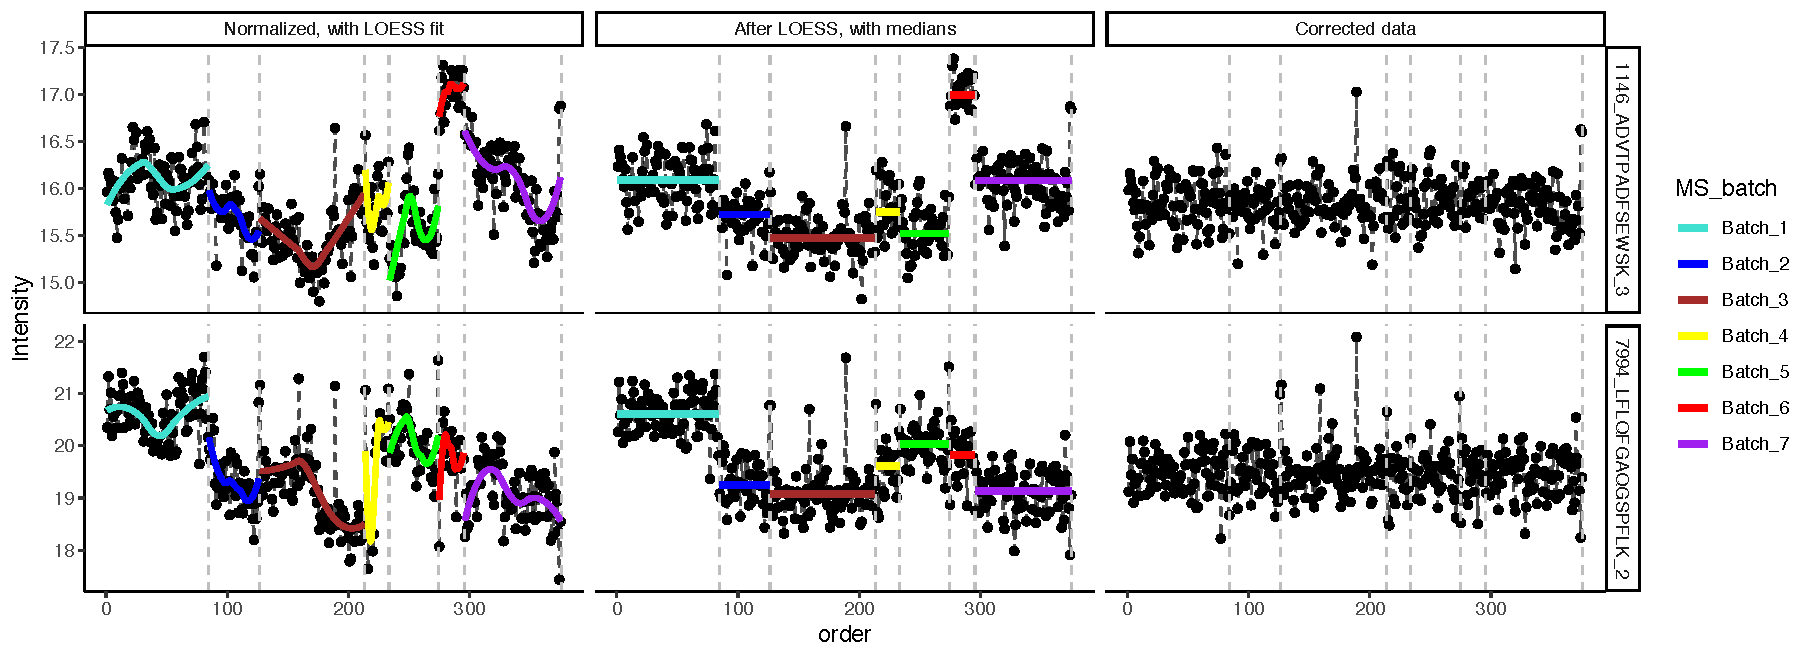
\includegraphics[width=\textwidth]{figures/Fig5_batch_correction.pdf}
	
	\caption{\textbf{Two-step correction of batch effects}  \\
		\footnotesize
		(A) Fitting a LOESS curve for every peptide in each batch and subtracting the fit; (B) Using medians for correction of the residual discrete batch effect; (C) The corrected data is more uniform and can now be used for downstream analysis. Data from the Aging mouse study.}
	\label{fig:batch_fig5_batchCorrection}
\end{figure}

The goal of batch effects correction is to alleviate the residual bias after normalization. In most cases, normalization significantly reduces the unwanted variance (see representative peptides in \textcolor{red}{Supplementary Fig. 3C}), and, as in the InterLab study, might somtimes be the only required adjustment. However, in many cases the batch effects diagnostic procedures described in the previous section will reveal that individual features are differentially affected by batch effects even after normalization (Figure~\ref{fig:batch_fig3_diagnostics}D and Figure~\ref{fig:batch_figS2_PanCancer}C). Indeed, batch effects correction is typically applied at the feature-level.

Feature-level bias in proteomics can be of various nature. In the Aging mouse data, the peptides manifest an order-specific, continuous bias, while the PanCancer data exhibits discrete shifts. The latter can be corrected with methods established by the genomics community, whereas the former is typical of large MS-based proteomic experiments and will therefore be discussed in more details in the following paragraphs.

In MS-based proteomics, samples are analyzed sequentially typically using an on-line chromatographic system directly coupled to a mass spectrometer. Various components of this system are susceptible to degradation of performances over time (e.g. changes in the properties of the chromatographic material, emitter degradation, contamination of MS lenses, mass calibration drift, ...). Various factors, such as sample quality and composition, can contribute to the speed of this degradation. However, even under best case conditions, one can expect to see noticeable degradation after a few hundred runs. Therefore, continuous batch effects associated with signal drift are characteristic of MS-based proteomics. They are also increasing in importance as they are particularly relevant in large scale studies. For instance, the Aging mouse study was comprised of almost 400 samples and therefore had to be split into 7 MS measurement batches, each with a unique signal drifting pattern to it.

To address this complex bias, we have developed a two-step batch correction procedure shown in \textcolor{red}{Figure~\ref{}}. In the first step, MS signal drift is corrected based on non-linear curve fitting. As a curve-fitting algorithm, we have chosen LOESS, as it combines computational simplicity with relative flexibility of the fit characteristics. The procedure runs as follows: for each peptide and each batch, a unique curve is fit (Figure~\ref{fig:batch_fig5_batchCorrection}A), and then subtracted from the normalized intensity value in each sample, leading to measurements, whose median is different in each batch (Figure~\ref{fig:batch_fig5_batchCorrection}B). Second, after this initial correction a discrete batch effects correction procedure can be applied (e.g. median centering, ComBat, ...). In the Aging mouse (Figure~\ref{fig:batch_fig5_batchCorrection}C) and PanCancer studies we opted to use median centering at this stage. It should be noted that while this approach can cope with missing values, having a significant percentage of missingness will compromise its effectiveness. For more details on missing value problem see \hyperref[box:Box3_missingness]{Box 3 "Missing values"}.

When several batch factors affect the data (as diagnosed by PCA, Hierarchical clustering and/or PVCA), all factors should be accounted for during correction. This typically means that batch factors get combined. This however, is not always possible. In the Aging mouse study for instance, the two main technical factors, MS batch and digestion batch, were highly confounded. Thus, we opted to only correct for MS batch.

In conclusion, batch effect correction removes variance from known, annotated batch factors. Whether the adjustment procedures – normalization and batch effects correction – improved the data signal, remains however to be determined by a quality control step.


\subsection{Quality Control}
\begin{figure}[hbt]
	%\center
	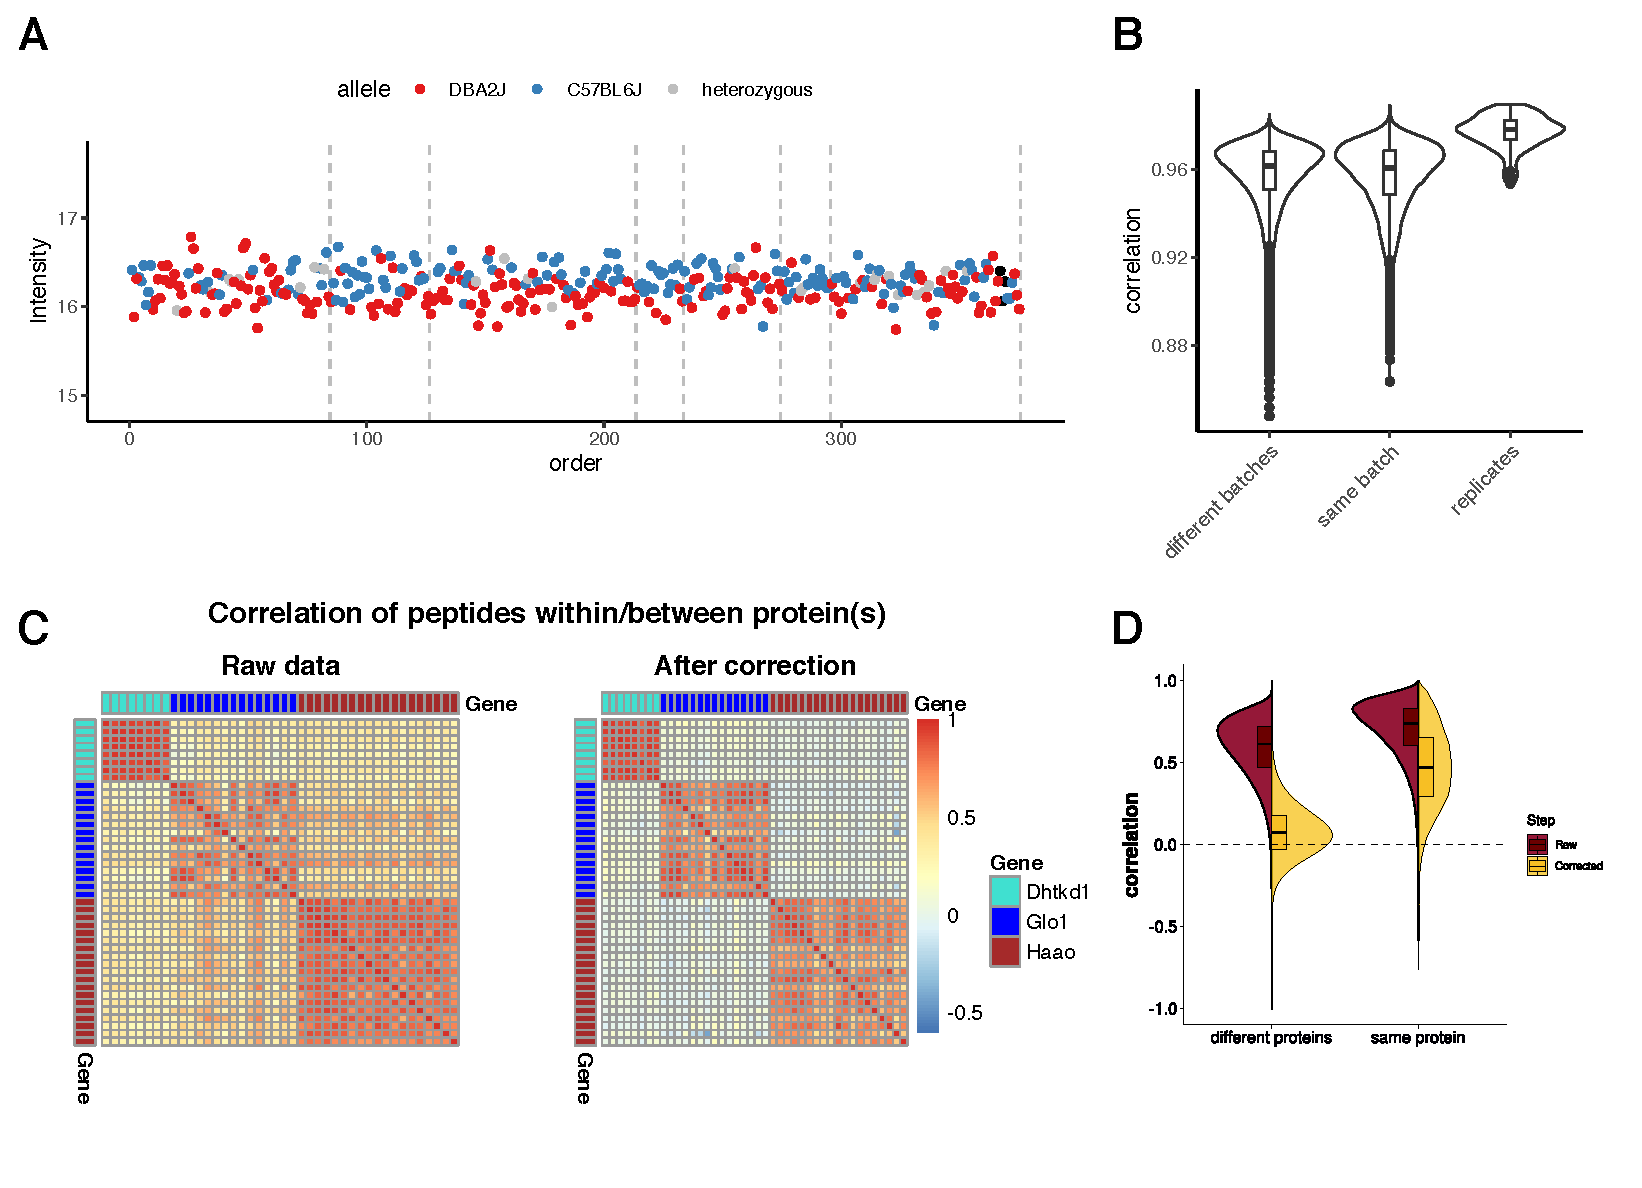
\includegraphics[width=\textwidth]{figures/Fig5_quality_control2.pdf}
	
	\caption{\textbf{Quality control of batch effects correction}  \\
		\footnotesize
		(A) Representative "Acads" protein QTL, that in corrected data demonstrates a clear allele separation; (B) Distribution of sample correlations - between batches, within batches and in replicated samples for corrected data; (C)  Heatmaps of peptide correlation for the proteins DHTKD1, GLO1 and HAAO, before and after correction: correlation is positive for all peptides in raw data, while after batch correction the correlation of unrelated peptides becomes close to zero; (D) Distribution of peptide correlation in raw data (brown) and in batch corrected data (yellow) for peptides from different proteins and peptides from the same protein: while same-protein peptide correlation is always higher than the correlation of unrelated peptides, the correlation of unrelated peptides approaches zero only after the correction.}
	\label{fig:batch_fig6_QualityControl}
\end{figure}


The main goal of the quality control step is to determine, whether the data quality has improved. There are two types of quality controls. Negative controls, signify that biases, detected during the initial assessment or diagnostic steps are no longer affecting the data. Positive controls indicate that the data quality has improved. Certain quality controls are a mixture of both types.

Examples of negative controls are the plots discussed in the diagnostics section like individual peptides plots, PCA, hierarchical clustering or PVCA. In most cases, these show that samples are no longer affected by batch-specific patterns (e.g. PanCancer study corrected Bovine peptides in Figure~\ref{fig:batch_figS2_PanCancer}E and F and hierarchical clustering in Figure~\ref{fig:batch_figS2_PanCancer}C and D).

It is common is to judge signal improvement by “better” clustering of biological groups, as seen on PCA, hierarchical clustering, or higher weight of that biological factor in PVCA. Unfortunately, this approach has serious pitfalls. First of all, it is a “self-fulfilling prophecy”. When variance is removed from technical factors, the relative weight of the remaining, biological, factors will increase. Second the actual differences in the proteomes of two biological states of interest (e.g. disease vs. healthy), might be too small to drive clustering. Thus, it’s not appropriate to state “the correction did not work” because the clustering by biological factors did not improve. Respectively, this approach also cannot be used to choose a normalization or correction procedure.

Generally speaking, clustering or PVCA, are valuable as negative controls. However one should resist the temptation of concluding, based on negative controls alone, that the overall data quality has been improved. For this purpose one should instead use positive controls.

Depending on the experimental setup, one can sometimes judge the data improvement through the presence of better biological signal. In the Aging mouse study, this can be achieved via known Quantitatative Trait Loci (QTL), particularly cis-QTLs (i.e. alleles of specific genes  affecting protein expression). As seen in Figure~\ref{fig:batch_fig6_QualityControl}A, certain proteins become clearly easier to separate and less biased than before the bias adjustment (compare to Figure~\ref{fig:batch_fig2_initAssessment}C). In addition to \textcolor{red}{XYZ} QTLs detectable in the raw data, an additional \textcolor{red}{ABC} alleles pass the significance threshold after normalization and a further \textcolor{red}{DEF} after batch correction. This essentially indicates that most of the batch effects are adjusted for at the normalization step, supporting the choice of normalization to be the only batch adjustment step.

Next we propose two positive control approaches, that can be used in almost any proteomic experimental context.


The first method is based on assessing sample proximity (proximity is commonly measured as correlation). 
Two comparisons are particularly important: 1) the comparison of correlation distributions for intrabatch and unrelated samples, which should be similar in unbiased data; 2) the comparison of correlation distributions for replicates and all other samples, which should be clearly skewed in favour of the replicates in unbiased data. Note that although individual replicates might have lower correlation than unrelated samples, as a distribution, replicate correlation has to be stronger. In the Aging mouse dataset these two comparisons can be seen pre- and post-adjustment in Figure~\ref{fig:batch_fig2_initAssessment}B and Figure~\ref{fig:batch_fig6_QualityControl}B. This approach and considerations can also be applied with different distance measures and visualizations. Figure~\ref{fig:batch_figS2_PanCancer}G and H demonstrate this concept on the PanCancer data using Manhattan distance and a dendrogram representation. These, proximity-based quality controls are universally  applicable to any dataset with replicated samples and batches.

The second method is based on assessing the proximity of feature sets. In bottom-up proteomics these are peptides or fragments. Similarly to the previous method, the distance between related peptides (i.e. belonging to a common protein) is expected to be smaller than the distance between unrelated ones.. This effect is true not only to selected proteins (Figure~\ref{fig:batch_fig6_QualityControl}C left) but also holds true for the whole proteome (Figure~\ref{fig:batch_fig6_QualityControl}D, dark brown). The correlation of unrelated peptides, however, gets much closer to zero after the correction (Figure~\ref{fig:batch_fig6_QualityControl}C right, and Figure~\ref{fig:batch_fig6_QualityControl}D yellow). Hence, before correction most of the peptide correlation was spurious.

In summary, through a combination of positive and negative quality controls, it is possible to assess improvements in data quality. It should however be stressed, that quality control methods are not criteria for choosing batch adjustment methods. Rather their purpose is to provide metrics to control the quality of the data before and after adjustment.

\section{Computational tools and analysis}

To facilitate the practical application of the steps and principles described in this manuscript, we have developed an R package, named "proBatch" and made it available in Bioconductor (https://bioconductor.org/packages/release/bioc/html/proBatch.html). proBatch wraps multiple established techniques for data transformation and visualization with proven utility in the adjustment of batch effects. 

The package has been designed based on the following principles to facilitate the construction of batch effect adjustment pipelines:

\begin{itemize}
    \item For each step of the workflow one or more functions are provided.
    \item The input to each function is standardized to a feature measurement table (e.g. peptide, protein, fragment, transition) and an annotation table with technical and biological factors.
    \item Consistent visual representation of factors at all steps of the analysis.
\end{itemize}

Note that we have also deliberately avoided the inclusion of an "adjust for batch effects" function to promote awareness of the properties of a particular dataset and to enable informed selection of appropriate data transformation methods.

We also make the code used for the analyses of the three case studies presented in this manuscript available on Github (https://github.com/symbioticMe/batch_effects_workflow_code). An accompanying docker container containing all the tools required to replicate the analyses is made available on Dockerhub (ADD_LINK).

\section{Discussion}

Large-scale proteomic studies, enabled by recent technological advances, unleashed the statistical power required for systems biology and translational medicine studies. However, great power comes with batch effects baggage. 

It is sometimes argued, that batch effects should not be corrected, but rather incorporated into the downstream analysis. For example, one way to account for batch effects in differential expression analysis using ANOVA is to use the batch as one of multiple factors affecting protein abundance. This approach is backed up with decades of statistical research and practice, but has a few practical downsides. First, for quantification methods, based on within-protein peptide correlation, unadjusted batch effects can compromise quantification via spurious peptide correlations. Second, incorporating batch effects in downstream analyses is not always straightforward (e.g. correlation network inference). This explains, why most large-scale studies opt for correcting batch effects and proceed with a “batch-free” dataset.

Another common advice regarding batch effects is to not correct them to avoid “flattening” of the signal. Typically, when significant hits disappear after batch correction, the biological groups were confounded with the batch factors. This is a serious experimental design error and can be prevented by balancing the biological groups between the expected batches. On the other hand, to account for hill defined batches (e.g. MS-batches) samples can be randomized.

Most methods for the identification and correction of batch effects in MS-based proteomics data can be borrowed from the genomics field. However, missing values represent a key distinction between the fields. These are often batch-associated and can cause established clustering and correction methods to fail. For example, missing values often lead to “uncorrectable” batch effects seen as batch clusters in PCA. This, however, is often due to filling the batch-specific missing values with zeros or small random numbers. Other methods, such as hierarchical clustering or ComBat, could potentially be adapted to account for the sparsity of proteomics data. Even so, proteomics, could benefit from the development of more methods robust against data missingness.

Specialized proteomics applications could also benefit from further batch adjustment methodological developments. In this manuscript we presented a workflow designed with DIA data in mind, due to its reproducibility and quantitative robustness in a large sample size setting. Since the protocol relies on having a quantitative data matrix with few assumptions on its structure, it is in principle also applicable to other quantitative proteomics workflows (e.g. TMT, label free, ...). However, proteomics applications incorporating affinity purification, size exclusion chromatography, PTM-centric protocols or subcellular fractionation are typically more heterogeneous. These dataset types will require additional efforts for batch effects characterization and correction.

In conclusion, mass spectrometry based proteomics has come a long way, and is still continuing to evolve. As throughput and reproducibility increase, so do batch effects-related issues. Hence, we expect experimental design and batch effects correction methods to also grow in importance and to take center stage in  large scale proteomics applications such as clinical proteomics and systems biology.


\section*{Supplementary files}
Links to the data files, proBatch code, manuscript code.

\section*{Contributions}

Contributions
J.~Č and P.~P. designed the analysis workflow and wrote the manuscript, E.~W. introduced multiple components in the workflow and made major contributions to the manuscript outline and text. J.~Č., C. ~L., E.~W. and V.~S. performed data analysis. J.~Č., C.~L. and P.~P. implemented back-end R functionality, E.~W. helped with the code testing. E.~W., T.~S. and B.~C. provided proteomic data and contributed to workflow conceptualization. M.~R.-M. provided critical input on the project and assisted in analysis pipeline design. P.~P. and R.~A. supervised the study.

\section*{Acknowledgements}
1. Guy who wrote "split violinplot" function. Qing Zhong and Rebecca Poulos for early feedback on the pipeline and all Aebersold lab for critical comments and questions.

\section*{Conflict of interest}
Authors declare no conflict of interests


\printendnotes

% Submissions are not required to reflect the precise reference formatting of the journal (use of italics, bold etc.), however it is important that all key elements of each reference are included.
\bibliography{batch_references}

\graphicalabstract{example-image}{Please check the journal's author guidelines for whether a graphical abstract, key points, new findings, or other items are required for display in the Table of Contents.}

\newpage
\section{Supplementary Material}
\beginsupplement

\begin{figure}
	\centering
	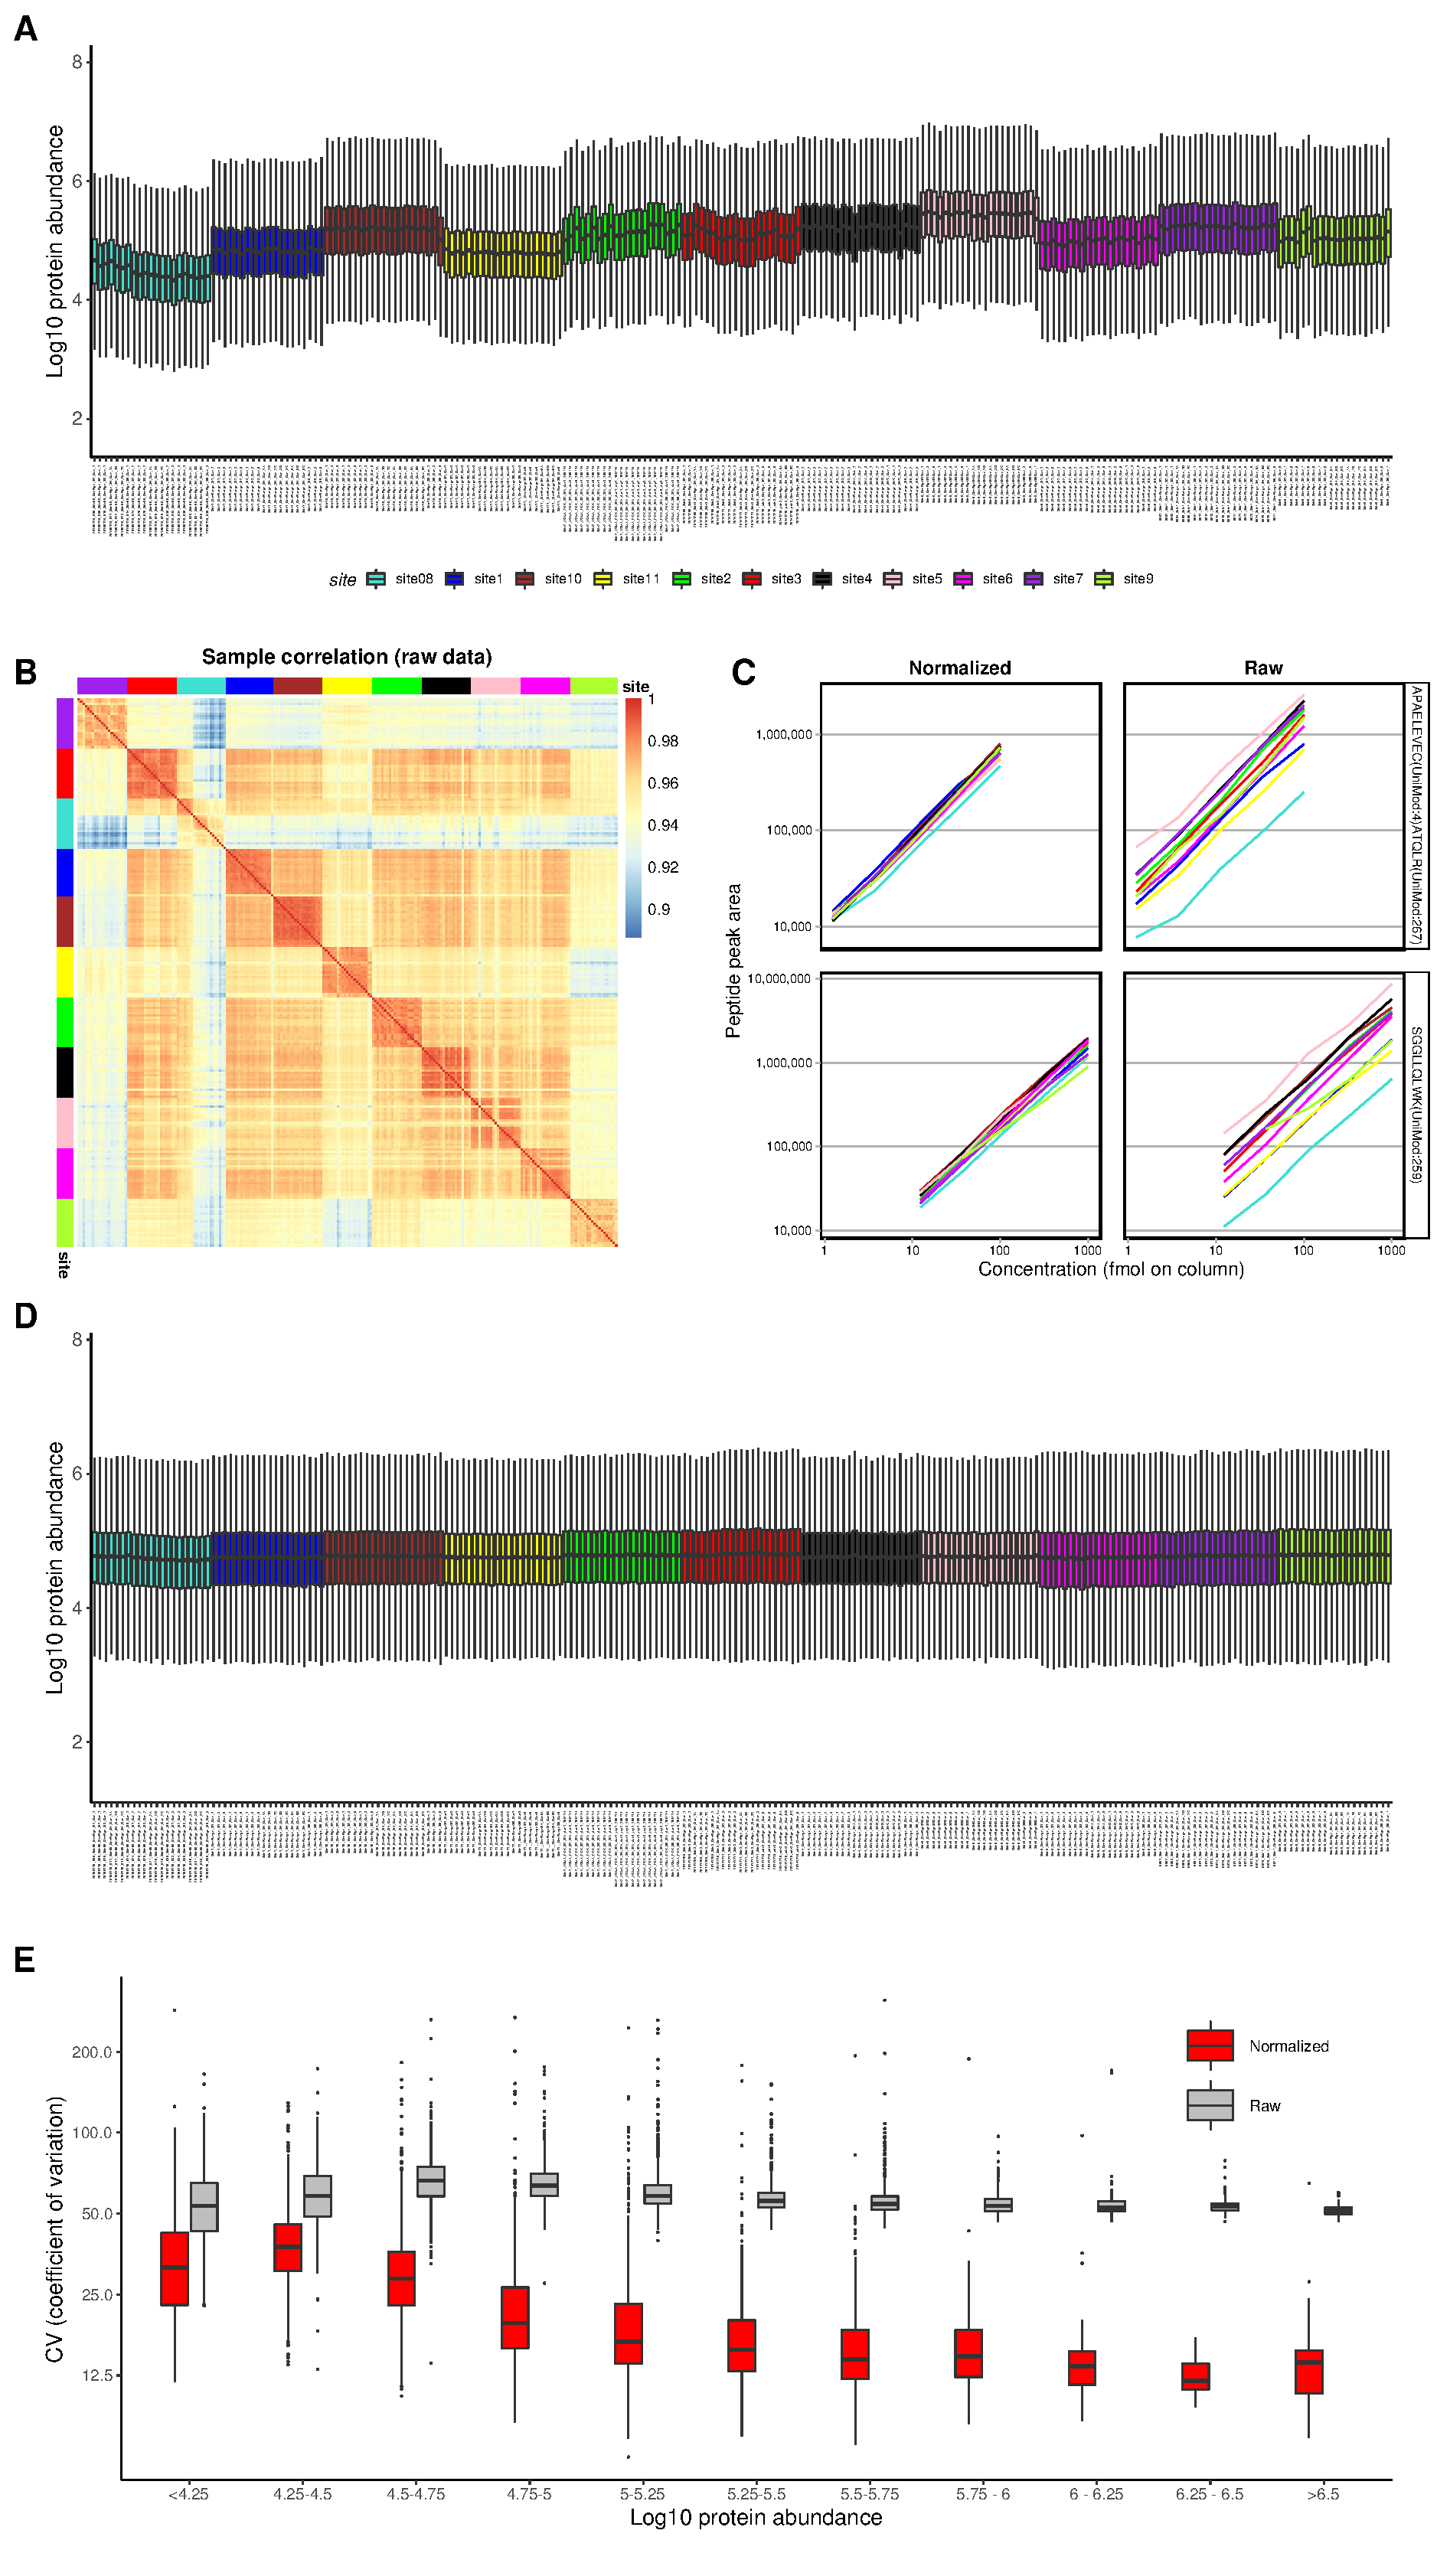
\includegraphics[width=\textwidth,height=.9\textheight,keepaspectratio]{figures/Supp_InterLab.pdf}
	\caption{\textbf{Batch effects in the InterLab study}\\
		 \footnotesize  (A) Boxplots of raw sample intensities colored by MS spectra acquisition sites; (B) Sample correlation heatmap, top row and left column colored by MS spectra acquisition sites, used as a quality control; (C) Comparison of two spike-in peptide quantification in raw and normalized data; (D) Boxplots of median-normalized sample intensities; (E) Quality control by comparing coefficient of variance (CV) for proteins, binned by Log10 abundance.}
	\label{fig:batch_figS1_InterLab}
\end{figure}

\begin{figure}
	%\center
	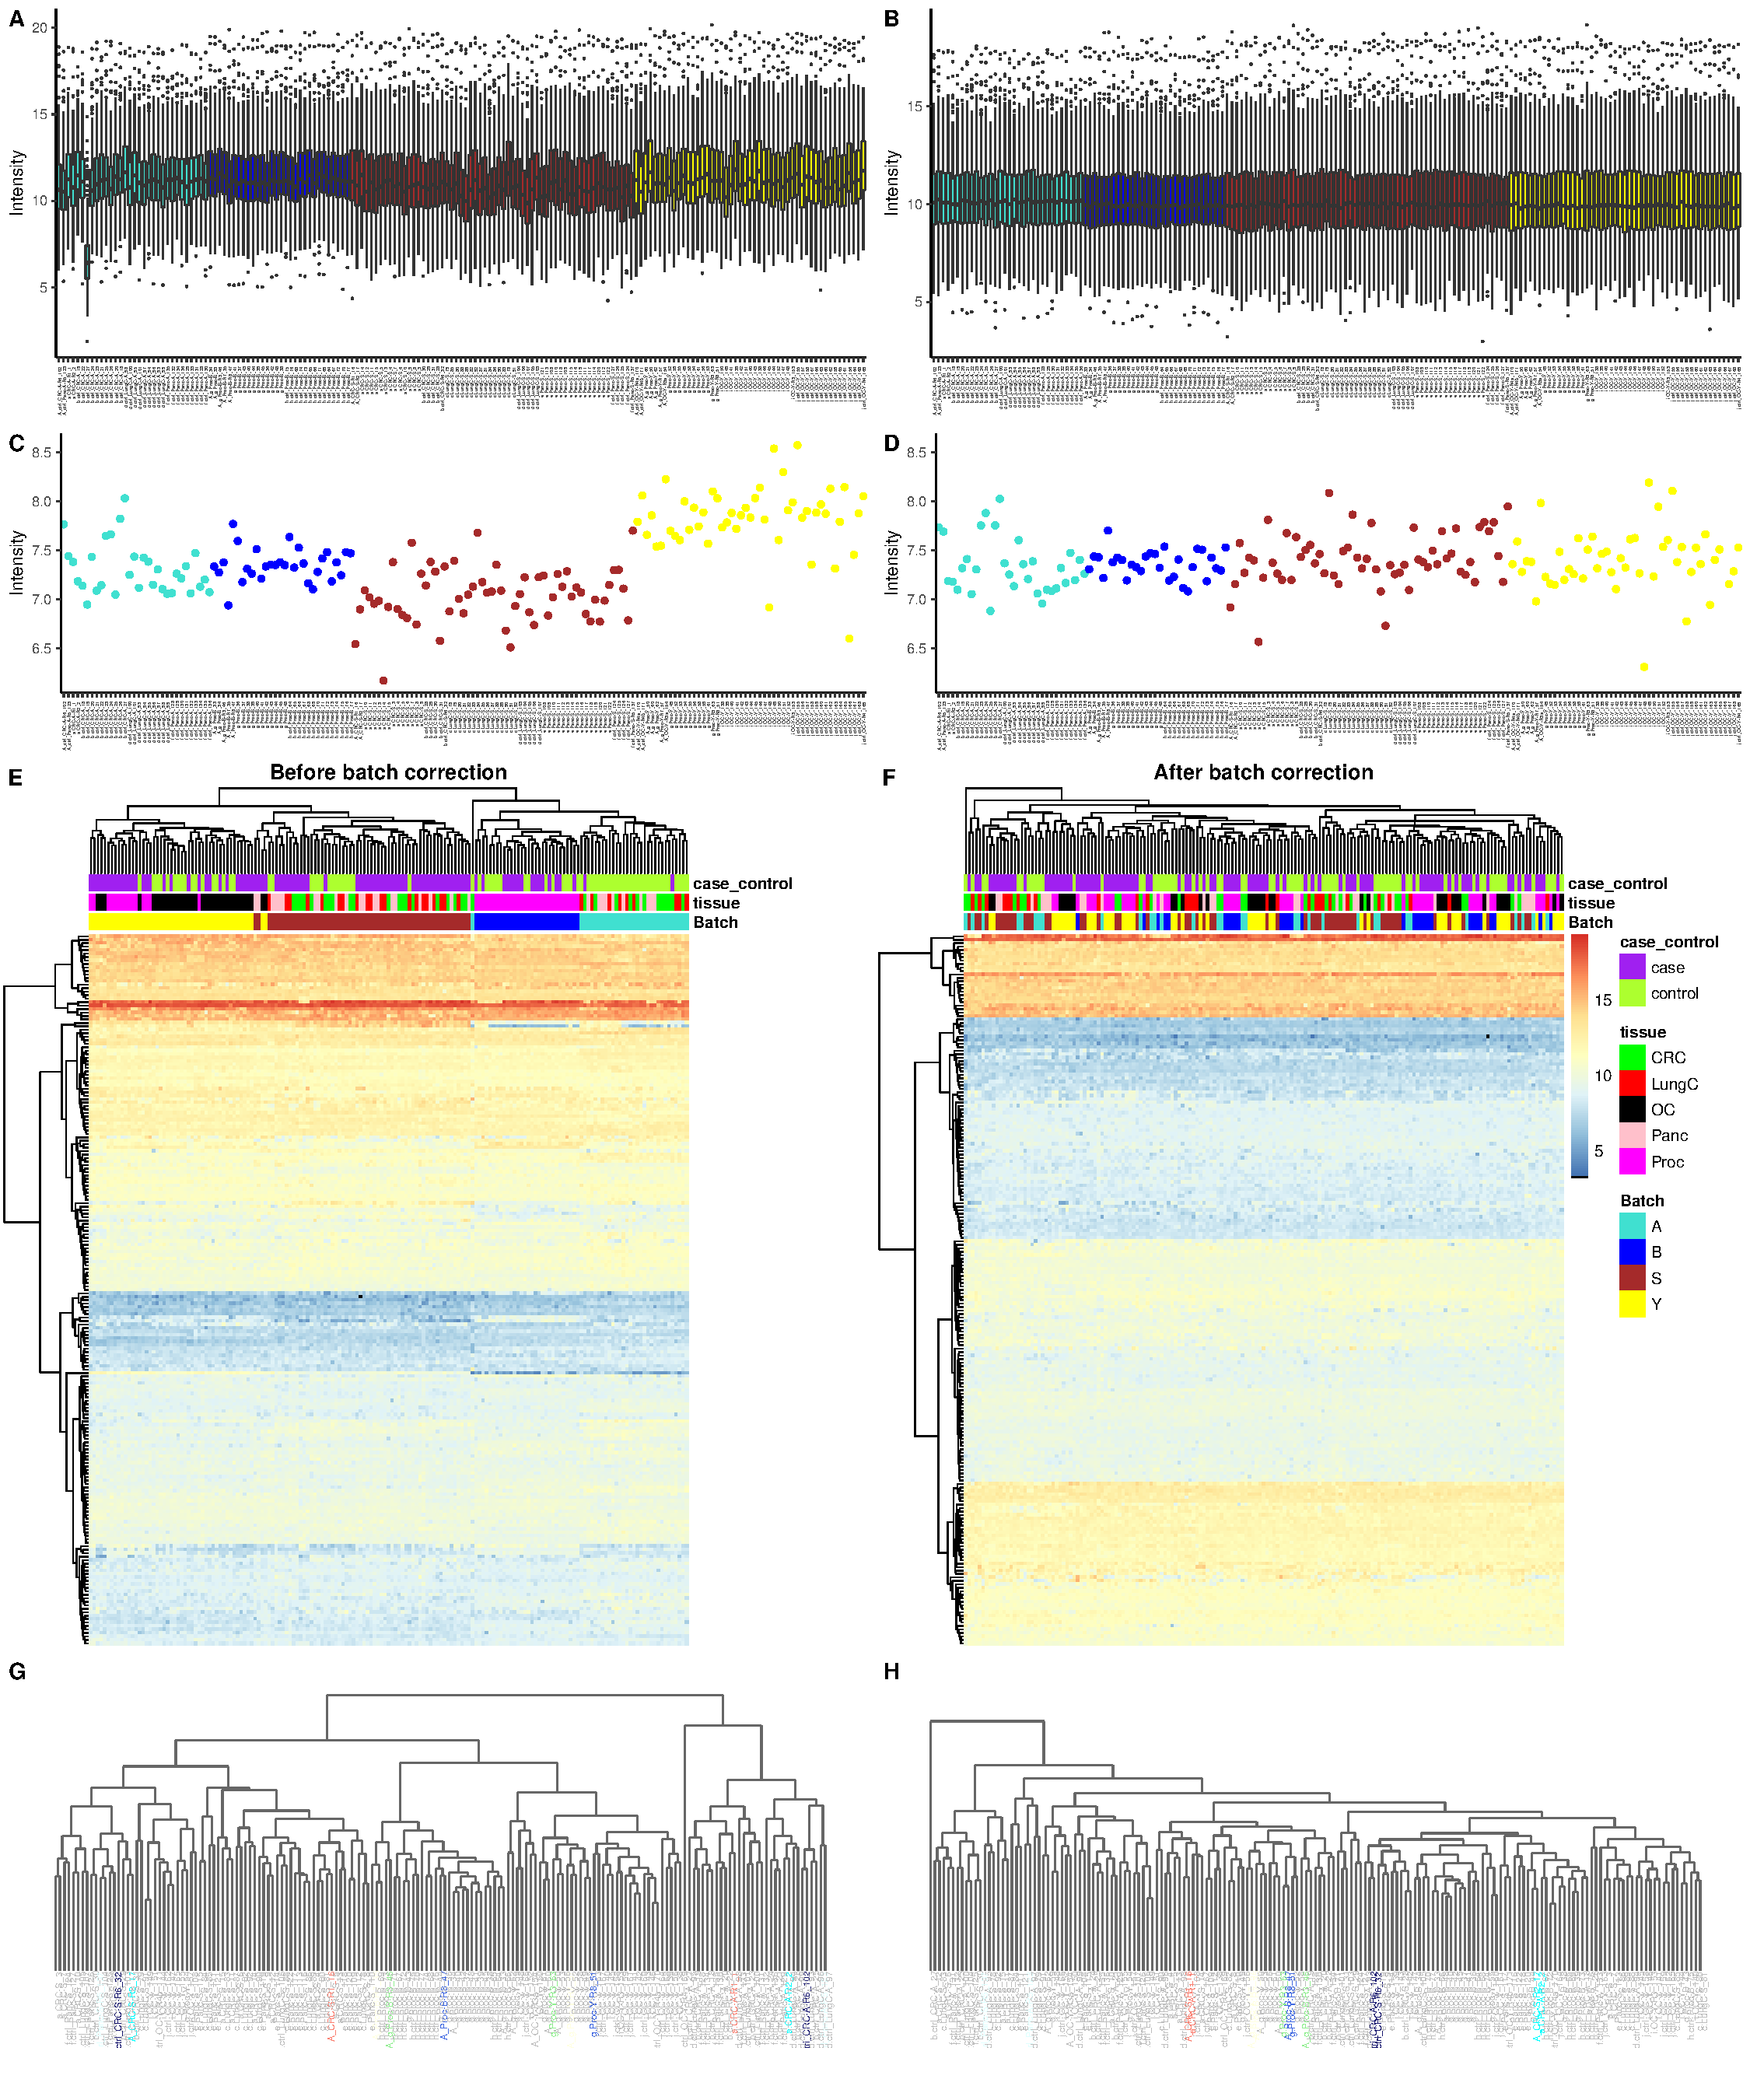
\includegraphics[width=\textwidth]{figures/Supp_Fig2_PanCancer}
	
	\caption{\textbf{Batch effects in the PanCancer study} \\
		\footnotesize (A) Boxplots of raw sample intensities colored by digestion batch; (B) Boxplots of normalized sample intensities colored by digestion batch; 
		(C) Intensity of spike-in Fetubin in raw data; (D) Intensity of spike-in Fetuin in batch corrected data; (E) Hierarchical clustering and heatmap of raw protein-level data; (F) Hierarchical clustering and heatmap of batch corrected protein-level data; (G) Hierarchical clustering of normalized data with Manhattan distance, with replicated samples colored; (H) Hierarchical clustering of batch corrected data with Manhattan distance, with replicated samples colored.}
	\label{fig:batch_figS2_PanCancer}
\end{figure}


\end{document}
